%  links for CASE 2016, http://case2016.org/  
% https://ras.papercept.net/conferences/scripts/login.pl      to submit
% https://ras.papercept.net/conferences/scripts/pdftest.pl  to test pdf

% obstacles: brown
% robots: blue

%(Note:   Similar games are SuperFruitfall and Denki Blocks). 


\documentclass[letterpaper, 10 pt, conference]{ieeeconf}
\IEEEoverridecommandlockouts
%\documentclass[12pt]{article}
%\usepackage{times}
\usepackage{calc}
\usepackage{url}
\usepackage{hyperref}
\hypersetup{
  colorlinks =true,
  urlcolor = black,
  linkcolor = black
}
\usepackage{graphicx}
\usepackage[cmex10]{amsmath}
\usepackage{bm}
\usepackage{amssymb}
\usepackage{rotating}


%\usepackage{xfrac}
\usepackage{nicefrac}
\usepackage{cite}
\usepackage[caption=false,font=footnotesize]{subfig}
\usepackage[usenames, dvipsnames]{color}
\usepackage{colortbl}
%\usepackage{caption}

%\usepackage{wrapfig}
\usepackage{overpic}
%\usepackage{subfigure}
%\usepackage{textcomp}
\graphicspath{{./pictures/pdf/},{./pictures/ps/},{./pictures/png/},{./pictures/jpg/},{./code/Data/}}
\usepackage{breqn} %for breaking equations automatically
\usepackage[ruled]{algorithm}
\usepackage{algpseudocode}
%\usepackage{algorithmic}
\usepackage{multirow}
\usepackage{todonotes}

%\newcommand{\todo}[1]{\vspace{5 mm}\par \noindent \framebox{\begin{minipage}[c]{0.98 \columnwidth} \ttfamily\flushleft \textcolor{red}{#1}\end{minipage}}\vspace{5 mm}\par}
% uncomment this to hide all red todos
%\renewcommand{\todo}{}

%% ABBREVIATIONS
\newcommand{\qstart}{q_{\text{start}}}
\newcommand{\qgoal}{q_{\text{goal}}}
\newcommand{\pstart}{p_{\text{start}}}
\newcommand{\pgoal}{p_{\text{goal}}}
\newcommand{\xstart}{x_{\text{start}}}
\newcommand{\xgoal}{x_{\text{goal}}}
\newcommand{\ystart}{y_{\text{start}}}
\newcommand{\ygoal}{y_{\text{goal}}}
\newcommand{\gammastart}{\gamma_{\text{start}}}
\newcommand{\gammagoal}{\gamma_{\text{goal}}}
\providecommand{\proc}[1]{\textsc{#1}}


\newcommand{\ARLfull}{Aero\-space Ro\-bot\-ics La\-bora\-tory }
\newcommand{\ARL}{\textsc{arl}}
\newcommand{\JPL}{\textsc{jpl}}
\newcommand{\PRM}{\textsc{prm}}

\newcommand{\CM}{\textsc{cm}}
\newcommand{\SVM}{\textsc{svm}}
\newcommand{\NN}{\textsc{nn}}
\newcommand{\prm}{\textsc{prm}}
\newcommand{\lemur}{\textsc{lemur}}
\newcommand{\Lemur}{\textsc{Lemur}}
\newcommand{\LP}{\textsc{lp}} 
\newcommand{\SOCP}{\textsc{socp}}
\newcommand{\SDP}{\textsc{sdp}}
\newcommand{\NP}{\textsc{np}}
\newcommand{\SAT}{\textsc{sat}}
\newcommand{\LMI}{\textsc{lmi}}
\newcommand{\hrp}{\textsc{hrp\nobreakdash-2}}
\newcommand{\DOF}{\textsc{dof}}
\newcommand{\UIUC}{\textsc{uiuc}}
%% MACROS


\providecommand{\abs}[1]{\left\lvert#1\right\rvert}
\providecommand{\norm}[1]{\left\lVert#1\right\rVert}
\providecommand{\normn}[2]{\left\lVert#1\right\rVert_#2}
\providecommand{\dualnorm}[1]{\norm{#1}_\ast}
\providecommand{\dualnormn}[2]{\norm{#1}_{#2\ast}}
\providecommand{\set}[1]{\lbrace\,#1\,\rbrace}
\providecommand{\cset}[2]{\lbrace\,{#1}\nobreak\mid\nobreak{#2}\,\rbrace}
\providecommand{\lscal}{<}
\providecommand{\gscal}{>}
\providecommand{\lvect}{\prec}
\providecommand{\gvect}{\succ}
\providecommand{\leqscal}{\leq}
\providecommand{\geqscal}{\geq}
\providecommand{\leqvect}{\preceq}
\providecommand{\geqvect}{\succeq}
\providecommand{\onevect}{\mathbf{1}}
\providecommand{\zerovect}{\mathbf{0}}
\providecommand{\field}[1]{\mathbb{#1}}
\providecommand{\C}{\field{C}}
\providecommand{\R}{\field{R}}
\newcommand{\Cspace}{\mathcal{Q}}
\newcommand{\Uspace}{\mathcal{U}}
\providecommand{\Fspace}{\Cspace_\text{free}}
\providecommand{\Hcal}{$\mathcal{H}$}
\providecommand{\Vcal}{$\mathcal{V}$}
\DeclareMathOperator{\conv}{conv}
\DeclareMathOperator{\cone}{cone}
\DeclareMathOperator{\homog}{homog}
\DeclareMathOperator{\domain}{dom}
\DeclareMathOperator{\range}{range}
\DeclareMathOperator{\sign}{sgn}
\providecommand{\polar}{\triangle}
\providecommand{\ainner}{\underline{a}}
\providecommand{\aouter}{\overline{a}}
\providecommand{\binner}{\underline{b}}
\providecommand{\bouter}{\overline{b}}
\newcommand{\D}{\nobreakdash-\textsc{d}}
%\newcommand{\Fspace}{\mathcal{F}}
\providecommand{\Fspace}{\Cspace_\text{free}}
\providecommand{\free}{\text{\{}\mathsf{free}\text{\}}}
\providecommand{\iff}{\Leftrightarrow}
\providecommand{\subinner}[1]{#1_{\text{inner}}}
\providecommand{\subouter}[1]{#1_{\text{outer}}}
\providecommand{\Ppoly}{\mathcal{X}}
\providecommand{\Pproj}{\mathcal{Y}}
\providecommand{\Pinner}{\subinner{\Pproj}}
\providecommand{\Pouter}{\subouter{\Pproj}}
\DeclareMathOperator{\argmax}{arg\,max}
\providecommand{\Aineq}{B}
\providecommand{\Aeq}{A}
\providecommand{\bineq}{u}
\providecommand{\beq}{t}
\DeclareMathOperator{\area}{area}
\newcommand{\contact}[1]{\Cspace_{#1}}
\newcommand{\feasible}[1]{\Fspace_{#1}}
\newcommand{\dd}{\; \mathrm{d}}
\newcommand{\figwid}{0.22\columnwidth}
\newcommand{\TRUE}{\textbf{true}}
\newcommand{\FALSE}{\textbf{false}}
\DeclareMathOperator{\atan2}{atan2}


\newtheorem{theorem}{Theorem}
\newtheorem{definition}[theorem]{Definition}
\newtheorem{lemma}[theorem]{Lemma}
\begin{document}

%%%%%%%%%%%%%% For debugging purposes, I like to display the TOC
%    \tableofcontents
%    \setcounter{tocdepth}{3}
%\newpage
%\mbox{}
%\newpage
%\mbox{}
%\newpage

%%%%%% END TOC %%%%%%%%%%%%%%%%%%%%%%%%%%%%%%%%%%%%%%%

\title{\LARGE \bf 
Object Manipulation and Position Control \\Using a Swarm With Global Inputs
%Force and Torque Control using a Swarm With Global Inputs
}
\author{Shiva Shahrokhi and  Aaron T. Becker%, 
\thanks{{S. Shahrokhi and A. Becker are with the Department of Electrical and Computer Engineering,  University of Houston, Houston, TX 77204-4005 USA {\tt\small  \{sshahrokhi2, atbecker\}@uh.edu}
}
} %\end thanks
} % end author block
\maketitle

\begin{abstract}
Swarms of micro and nano robots take advantage of the power of volume to achieve, otherwise unfeasible for individual robots, tasks such as targeted drug delivery and micro scale manufacturing. However, due to their minuscule size, micro robots cannot contain onboard processing for autonomy nor onboard power. One solution is to control the micro robots with an external signal, our global variable input, such as a magnetic field. The main challenges to controlling a swarm of robots with only global control inputs are the swarm?s under-actuated characteristic, the fluctuating number of robots in contact with the object and with other robots, and the robot?s tendency to separate from the swarm. Addressing the challenges stated above, this work presented controllers and algorithms for steering such a swarm to manipulate objects. Previous work showed that by controlling the mean and variance of the swarm, the swarm can manipulate convex polygonal objects through a simple maze. The remaining key challenge in object manipulation with a swarm is torque control. In addition to manipulating objects, torque control is also necessary for aligning sensors and emitters, and redirecting incoming signals. This work proved that swarms can execute torque control and presented algorithms to automate the use of torque control. Included in this paper, our experiments showed a swarm of 97 robots successfully manipulating rectangles by using autonomous torque control.

%
%Micro- and nano-robots can be manufactured in large numbers. Large numbers of micro robots are required in order to deliver sufficient payloads, but the small size of these robots makes it difficult to perform onboard computation.  Instead, these robots are often controlled by a global, broadcast signal. 
%In our previous work we focused on a block-pushing task, where a swarm of robots pushed a larger block through a 2D maze. One surprising result was that humans that only knew the swarm's mean and covariance completed the task faster that humans who knew the position of every robot~\cite{Becker2013b}. 
%Inspired by that work, we proved that we can control the mean position of a swarm and that with an obstacle we can control the swarm's position variance ($\sigma_x$ and $\sigma_y$). 
%We then wrote automatic controllers which could complete a block pushing task, but these controllers had some limitations~\cite{ShahrokhiIROS2015}. 
%One of the limitations was that we could only compress our swarm along the world $x$ and $y$ axes, and could not navigate workspaces with narrow corridors with other orientations. 
%One solution to these problems would be a controller that regulates the swarm's position covariance, $\sigma_{xy}$. 
%For controlling $\sigma_{xy}$, we prove that the swarm position covariance $\sigma_{xy}$ is controllable given boundaries with non-zero friction. 
%We then prove that two orthogonal boundaries with high friction are sufficient to arbitrarily position a swarm of robots. 
%We conclude by designing controllers that efficiently regulate $\sigma_{xy}$.
\end{abstract}

%TODO: new outline

%%%%%%%%%%% PAPER OUTLINE
% INTRODUCTION, Related work
%      micro/nano applications
%	open questions in swarm control
% 	difficulties in obtaining experimental data
% Theory:
%% Wall friction shape
%% Control 2 robots
% Simulation:
%% Use wall friction to control covariance 1. Make variances small(feedback), 2. Move Swarm to wall, 3. drag out swarm to achieve covariance(feedback) 4. Move to goal.
%% Algorithm to control position of 2 robots using friction
%%%%%%% Algorithm to control position of n robots using friction
% Experiment
%% Use wall friction to control covariance
%% Algorithm to control position of 2 robots using friction
%%Future Work

%%%%%%%%%%%%%%%
%\todo{image 1 should be the kilobots pushing an interesting object.  Current images 1 and 2 are not attractive, have the same caption, and the robots look like ellipses}
\section{Introduction}\label{sec:Intro}
Micro-robots can be manufactured in large numbers.
Our vision is for large swarms of robots to be remotely guided 1) through the human body, to cure disease, heal tissue, and prevent infection and 2) ex vivo to assemble structures in parallel. 
 For each application, large numbers of micro robots are required  to deliver sufficient payloads, but the small size of these robots makes it difficult to perform onboard computation.  Instead, these robots are often controlled by a global, broadcast signal. 
 Future implementations require control techniques that can reliably exploit large populations despite significant under-actuation.  
 

\begin{figure}
\begin{center}
	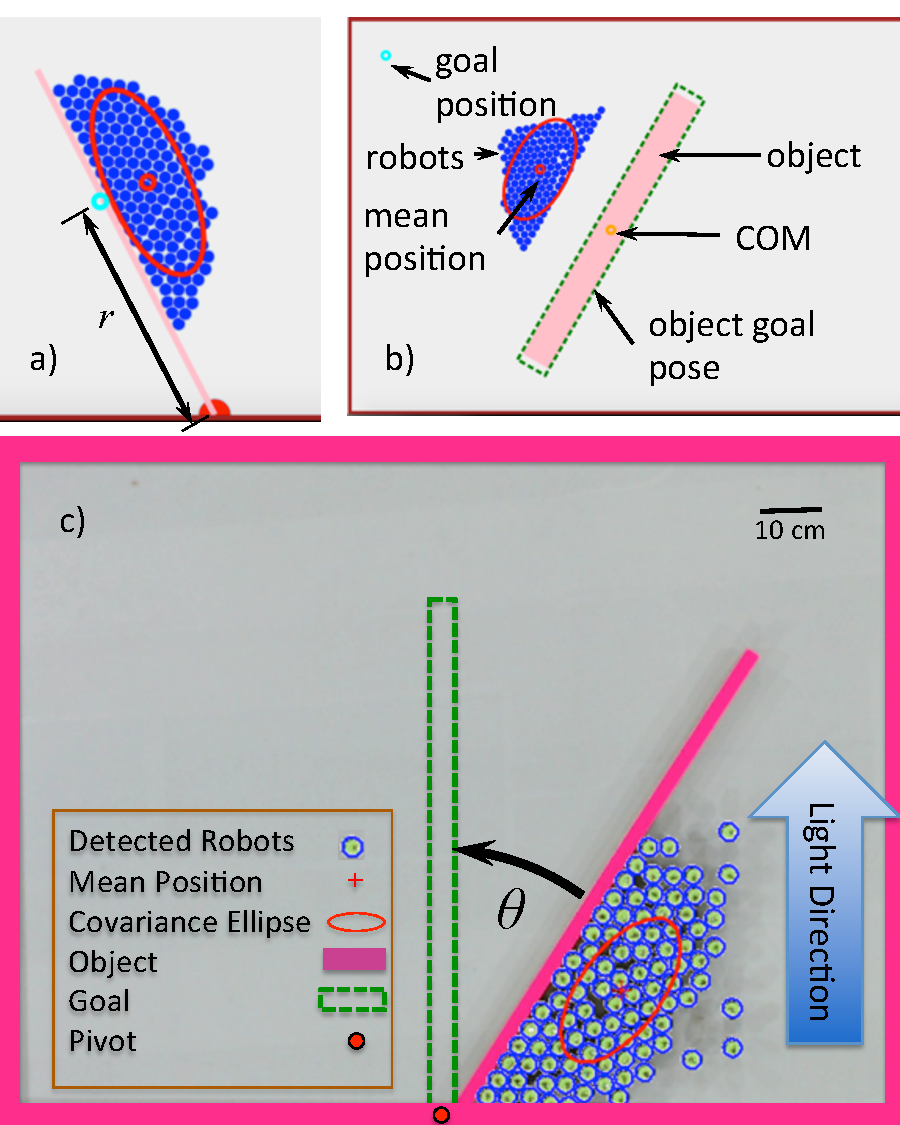
\includegraphics[width=.9\columnwidth]{CoverPhoto.pdf}
\end{center}
\vspace{-1em}
\caption{\label{fig:FirstImage}
Torque control of an object is essential for manipulating objects to their goal position  when there are narrow passageways and for aligning sensors, emitters, or other objects. 
This paper provides feedback control laws to apply torques and forces using a highly under-actuated system where all 
robots are controlled globally by the same input. 
(a) Simulation of robots exerting torque on a hinged ``door''.
(b) Simulation of swarm orientation manipulation.
(c) 97 hardware robots applying torque to an object. These robots have light sensors and are programmed to move toward the brightest light in the room.  This light is a shared control input that operates globally on the swarm. A full resolution video is available at:~\cite{ShahrokhiTorqueVideo}
}
\vspace{-1em}
\end{figure}


%One surprising result was that humans that only knew the swarm's mean and covariance completed the task faster that humans who knew the position of every robot~\cite{Becker2013b}. Our previous work focused on a block-pushing task, where a swarm of robots pushed a larger block through a 2D maze. 
Previous work proves that the mean position of a swarm is controllable and that, with an obstacle, the swarm's position variance orthogonal to rectangular boundary walls  is also controllable
(these are $\sigma_x^2$ and $\sigma_y^2$ for a workspace with axis-aligned walls). 
The usefulness of these techniques was demonstrated by several automatic controllers. One controller steered a swarm of robots to push a larger block through a 2D maze~\cite{ShahrokhiIROS2015}. 
We also showed methods to control a swarm's position covariance to enable the swarm to navigate through a workspaces with narrow corridors.  
However, object manipulation often also requires controlling torque on an object, for example changing the orientation of an object with a large aspect ratio to thread through narrow corridors.
Torque control  is also necessary for a variety of alignment tasks including retroreflectors, and targeted radiation therapy.

Accurate torque control is difficult.
A swarm with $n$ agents has $2n$ degrees of freedom.  
The swarm, when steered toward an object, begins interacting with the object at different times. 
The number of robots touching this object as a function of time is difficult to predict and often impossible to directly measure.
Stochastic effects make long-term prediction challenging.
Even when it is possible to predict which agents will hit the object first, as agents interact with the object, the swarm's configuration changes.
The challenge is not only limited to swarm-object interaction, but also to swarm-swarm interactions when the swarm self-collides  or is split into multiple components. 
As a result, the force the swarm will exert on the object is not easy to predict.
%Predicting the force a swarm exerts on an object requires knowing the location of every robot in contact with the object. 
This information is often hard to gather, because remote sensing of tiny particles is difficult.
Particles may be smaller than the minimum resolution of MRI, PET, and ultrasound, but these sensing modalities can still return aggregate data.
From this aggregate data,  some statistics---including mean and variance---are easy to obtain. 
Rather than design open-loop algorithms, this paper focuses on feedback control strategies using just two statistics of the swarm, the mean and variance of the swarm's position.


Fig. 1 illustrates the torque control using 97 kilobots, as well as two simulation snapshots of torque and orientation control.

%This paper first discusses the ways that we can control torque of an object in Section ~\ref{sec:theory}. Then it introduces algorithms for torque control in Section ~\ref{sec:simulation}. We show that algorithms work in Section ~\ref{sec:expResults} on 100 kilobots.

%For controlling $\sigma_{xy}$, we prove that the swarm position covariance $\sigma_{xy}$ is controllable given boundaries with non-zero friction. 
%We then prove that two orthogonal boundaries with high friction are sufficient to arbitrarily position a swarm of $n$ robots. 
%We conclude by designing controllers that efficiently regulate $\sigma_{xy}$.


%This paper
%(1) proves that the swarm position covariance $\sigma_{xy}$ is controllable given boundaries with non-zero friction,  %where do we do this?
%(2) proves that two orthogonal boundaries with high friction are sufficient to arbitrarily position two robots, 
%(3) proves that two orthogonal boundaries with high friction are sufficient to arbitrarily position a swarm of $n$ robots, 
%(4) shows full-state position control with 2 or more robots using  extensive simulations, and
%(5) demonstrate covariance control on our hardware platform with a large number of hardware robots.
%TODO JOURNAL: design controllers that efficiently regulate $\sigma_{xy}$.
%TODO JOURNAL: We will design Lyapunov-inspired controllers for $\sigma_{xy}$ to prove controllability. 
%TODO JOURNAL:  and rank controllability as a function of friction.
% TODO: JOURNAL: and vary wall friction by laser-cutting boundary walls with a variety of profiles. 







% Our paper is organized as follows.  After a discussion of related work in Section \ref{sec:RelatedWork}, we describe our experimental methods for an online human-user experiment in Section \ref{sec:expMethods}.  We report the results of our experiments in Section \ref{sec:expResults}, discuss the lessons learned in Section \ref{sec:discussion}, and end with concluding remarks in Section \ref{sec:conclusion}.



%%%%%%%%%%%%%%%

%%%%%%%%%%%%%%%%%%%%%%%%%%%%%%%%%%%%%%%%%%%%%%%%%%%%%%%%%%%
\section{Related Work}\label{sec:RelatedWork}
%%%%%%%%%%%%%%%%%%%%%%%%%%%%%%%%%%%%%%%%%%%%%%%%%%%%%%%%%%%

Unlike \emph{caging} manipulation, where robots form a rigid arrangement around an object~\cite{Sudsang2002,Fink2007}, our swarm of robots is unable to grasp the blocks they push, and so our manipulation strategies are similar to \emph{nonprehensile manipulation} techniques, e.g.~\cite{Lynch1999}, where forces must be applied along the center of mass of the moveable object. 


Robotic manipulation by pushing has a long and successful history\cite{Lynch1999,Lynch1996,Akella2000,Bernheisel2006}.  Key developments introduced the notion of stable pushes and a friction cone.  A \emph{stable push} is a pushing operation by a robot with a flat-plate pushing element in which the object does not change orientation relative to the pushing robot\cite{Lynch1999}.  The \emph{friction cone} is the set of vector directions a robot in contact with an object can push that object with a stable push.
Stable pushes can be used as primitives in an rapidly-expanding random tree to form motion plans.
A key difference is that our robots are compliant and tend to flow around the object, making this similar to fluidic trapping~\cite{Armani2006,Becker2009}.  
%\subsection{Block-pushing and Compliant Manipulation}

While ferrous particles tend to clump in a magnetic field, the magnetotactic bacteria of~\cite{martel2015magnetotactic,ou2012motion} are directed by the orientation of the magnetic field and do not suffer from magnetic aggregation.

Controlling the \emph{shape}, or relative positions, of a swarm of robots is a key ability for a myriad of applications.  Correspondingly, it has been studied from a control-theoretic perspective in  both centralized, e.g. virtual leaders in \cite{egerstedt2001formation}, and decentralized approaches, e.g. decentralized control-Lyapunov function controllers in~\cite{hsieh2008decentralized}. Most approaches assume a level of intelligence and autonomy in the individual robots that exceeds the capabilities of current micro- and nano-robots~\cite{martel2015magnetotactic,Xiaohui2015magnetiteMicroswimmers}.
Instead, this paper focuses on centralized techniques that apply the same control input to each member of the swarm, as in~\cite{Becker2013b}.





%
%More research has focused on generating artificial force-fields.  Applications have included techniques to design shear forces to a single object for sensorless manipulation~\cite{sudsang+2001:for}.  
%   Vose et al.\ demonstrated a collection of 2D force fields generated by 6DOF vibration inputs to a rigid plate~\cite{Vose2009a,vose2012sliding}.  This collection of force fields, including shear forces, could be used as a set of primitives for motion control for steering the formation of  multiple objects.
%   
%   %Flow in a pipe or body lume



%\subsection{Global-control of micro- and nanorobots} %\cite{Peyer2013,Shirai2005,Chiang2011}. 
%We are particularly motivated by harsh constraints in micro- and nanorobotic systems.  
%Small robots are often powered and steered by a global, broadcast control signal.  Examples include \emph{scratch-drive microrobots}, actuated and controlled by a DC voltage signal from a substrate \cite{Donald2006,Donald2008};  \emph{light-driven nanocars}, synthetic molecules actuated by a specific wavelength of light~\cite{Chiang2011},
% %magnetic structures  with different cross-sections that could be independently steered \cite{Floyd2011,Diller2013};   
% \emph{MagMite} microrobots with different resonant frequencies controlled by a global magnetic field \cite{Frutiger2008}; and  magnetically controlled nanoscale helical screws \cite{Tottori2012,Peyer2013}. Large numbers of robots can be constructed, but the user interaction required to individually control each robot scales linearly with robot population.   
%Instead, user interaction is often constrained to modifying a global input: while one robot is controlled, the rest are ignored. Making progress in targeted therapy and swarm manipulation requires the coordinated control of large robot populations.
%
%\subsection{Human user studies with large swarms}
%There is currently no comprehensive understanding of user interfaces for controlling multi-robot systems with massive populations~\cite{Nunnally2012HSI}.  
%Our previous work with over a hundred hardware robots and thousands of simulated robots~\cite{Becker2013b} demonstrated that direct human control of large swarms is possible. Unfortunately, the logistical challenges of repeated experiments with over one hundred robots prevented large-scale tests. To gather better data, we designed \href{http://www.swarmcontrol.net/show_results}{\emph{SwarmControl.net}}, a large-scale online game to test how humans interact with large swarms~\cite{Becker2014e}.  Our goal was to test several scenarios involving large-scale human-swarm interaction, and to do so with a statistically-significant sample size. These  experiments showed that numerous simple robots responding to global control inputs are directly controllable by a human operator without special training, and that the visual feedback of the swarm state should be very simple in order to increase task performance. \href{https://github.com/crertel/swarmmanipulate.git}{All code}~\cite{Chris-Ertel2013}, \href{http://www.swarmcontrol.net/show_results}{and experimental results} were posted online. The current paper presents motion primitives and an automatic controller that solves one of the games from \href{http://www.swarmcontrol.net/task/varying_visualization}{SwarmControl.net}.
%
%

%
%Our $n$-robot system with 2 control inputs and 4$n$ states is inherently under-actuated, and superficially bears resemblance to compliant, under-actuated manipulators~\cite{odhner2014compliant,deimel2014novel}.  Like these manipulators, the swarm conforms to the object to be manipulated.  However our swarm lacks the restoring force provided by flexures in \cite{odhner2014compliant} and the silicone in \cite{deimel2014novel}.  Our swarm tends to disperse itself, so we require  artificial forces, such as the variance control primitives in Section \ref{sec:VarianceControl},
% to regroup the swarm.

%Strategies based purely on particle flow also exist~\cite{Sugawara2012}, but these works 

%Manipulation by caging~\cite{Sudsang2002}

%We can also use a large population of robots for traditional nonprehensile tasks, such as transporting objects using the flow of the robots \cite{Sugawara2012}, and manipulating an object too heavy for a single robot. Our control formulation enables efficient control of this kind of transport.

%\subsection{Human-Swarm Interaction}
%Olson and Wood studied human \emph{fanout}, the number of robots a single human user could control~\cite{Jr2004}.  %Studied as a key aspect of human-robot interaction, 
%They postulated that the optimal number of robots was approximately  the autonomous time  divided by the interaction time required by each robot.  Their sample problem involved a multi-robot search task, where users could assign goals to robots.  Their user interaction studies with simulated planar robots  indicated a \emph{fanout plateau} of about 8 robots, after which there were diminishing returns.   They hypothesize that the location of this plateau is highly dependent on the underlying task, and our work indicated there are some tasks without plateaus. % (Lemmings is an example of this as well, for systems with autonomy
%Their research investigated robots with 3 levels of autonomy.  We use robots without autonomy, corresponding with their first-level robots.
%
%% Removed this -- 
%%Chen, Barnes, and Harper-Sciarini published a review of supervisory control but emphasized high levels of autonomy, using the 10-level taxonomy given by \cite{Parasuraman2000}.  The direct control techniques this paper examines are the lowest level.
%
%Squire, Trafton, and Parasuraman designed experiments showing that user-interface design had a high impact on the task effectiveness and the number of robots that could be controlled simultaneously in a multi-robot task \cite{Squire:2006:HCM:1121241.1121248}.
%
%A number of user studies compare methods for controlling large swarms of simulated robots, for example \cite{bashyal2008human,kolling2012towards,de2012controllability}.  These studies provide insights but are limited by cost to small user studies; have a closed-source code base; and focus on controlling intelligent, programmable agents.  
%For instance \cite{de2012controllability} was limited to a pool of 18 participants,  \cite{bashyal2008human} 5, and \cite{kolling2012towards} 32.
%	Using an online testing environment, we conduct similar studies but with much larger sample sizes.


%In our previous work with robots that can be modeled as nonholonomic unicycles~\cite{Becker2012k}, we showed that an inhomogeneity in turning speed is enough to make even an infinite number of robots controllable with regard to position. 
%While these approaches theoretically scale to large populations, they also require both excellent state estimation and heterogeneous robots. 

%For micro- and nanorobotics, the marginal cost of producing one additional robot is astonishingly small.  While some microrobots are individually fabricated \cite{Tottori2012}, others are fabricated using MEMS techniques \cite{Donald2008}, and these dies could be tiled to produce multiple copies.  Nanocars are exemplary of this diminishing marginal cost.  Nanocars are synthetic molecules with integrated axles, rolling wheels, and light-driven motors developed by Tour et al.\cite{Chiang2011}.  These  are routinely produced in quantities that are amazing---a batch  the size of an aspirin tablet  contained$~\approx4\times 10^{19}$ nanocars.  This dwarfs the total number of birds on the planet earth---some $3\times10^{11}$\cite{Gaston1997}. 
 %aspirin in US weighs 325 mg.
  %or the number of automobiles produced in the history of humankind
% http://www.virlab.virginia.edu/nanoscience_class/lecture_notes/Lecture_13_Materials/Tour%20on%20nanovehicles.pdf states:
%	On the other hand, nanocars synthesized in our laboratory
%	are each calculated to be approximately 3x6x4 nm in size, and
%	can be produced on the 30 mg scale (3.26x10^18 nanocars)
%	using small 100 ml laboratory reaction flasks, or more
%	nanocars than the number of automobiles made in the
%	history of the world (63 million automobiles were produced
%	in 2005). It would take 30 nanocars, side by side, to span the
%	90 nm width of a small line in the most advanced logic
%	chip being made today
% The motorized nanocar can be synthesized in 12 steps with an overall yield of 5\%,  An electrically driven one is \cite{Kudernac2011}
%Biological agents, including the magnetically controlled ciliate protozoa studied by A. Julius~\cite{Ou2012, Ou2012a} and the magnetotactic bacteria studied by Martel~\cite{Felfoul2011}can be grown or purchased in large numbers.
% According to a scientific study of trace elements in hair, a single strand of hair 4 1/2 inches in length weighs, on average, 0.62 milligram, with weights varying from 0.25 milligram to just under 1 milligram.
%mosquito weight = and weight up to 2.5 milligrams
%Read more: How much does one strand of human hair weigh? | Answerbag http://www.answerbag.com/q_view/2159502#ixzz2EUltJTAl
 

%
%Consider a collection of $n$ planar robots.  We  describe the configuration of the $i$-th robot by $q_i=[x_i,y_i]^\top$ and its configuration space by $\Cspace = \R^2$.  At the micro/nanoscale viscous effects dominate inertial forces~\cite{Purcell1977}, so our model ignores velocity and assumes in the absence of an external force, the robots stop moving.
% We describe the configuration of the environment by the magnitude of the force field $f = [f_x,f_y]\in\R^2$, which is assumed constant across the workspace.  The control inputs $u = [u_x,u_y]\in\R^2$ change this force field.
%\begin{align}
%\dot{x}_i &= f_x,&
%\dot{f_x} &= u_x,\nonumber \\
%\dot{y}_i &= f_y, &
%\dot{f_y} &= u_y. \label{eq:sysModel}
%\end{align}
%
%\todo{This model is key, because if we use impulsive inputs for $u_x$ and $u_y$, there are a number of tasks we can accomplish with a single input (e.g. 2,3,5,7 in Fig.~\ref{fig:boundaryManipulators}.)}

%In \cite{Becker2012} we proved that systems described by \eqref{eq:ensembleDynamics} can be approximately steered to arbitrary positions in $\R^2$.  In \cite{Becker2012k} we provided closed-loop controllers to drive $n$ robots to $n$ target positions.  For both works, the control laws apply even to an infinite robot continuum.  
%
%Unfortunately, in \cite{Becker2012}, we proved that the heading of the ensemble---the $\theta_i$ values---is not controllable.  The final heading of every robot in the ensemble is the scaled integration of all the turning control inputs, i.e.~ $\theta_i(T) = \theta_i(0) + \epsilon_i\int_0^T \omega(t)\,{\rm d}t$.  Instead of a full-state controller, we provided a control law that steered the position of each robot's center of rotation.  Our goal is to provide control algorithms for many robots with uniform inputs, with  application in trajectory following, manipulation, force-closure, and assembly at the micro- and nanoscale.  Regrettably, 
% being unable to control the heading of the robots makes many tasks difficult or impossible.  For instance, manipulation and assembly work without heading control requires that the robots be able to rotate in place and be circular, since we cannot specify the incident angle of the robots. %In practice, this limits the application of our work to circular or point robots. 
%As Lynch explained in \cite{Lynch1999}, pushing with a round object is inherently unstable.


%  Possible applications include using molecular robots as nanoscale transporters, to break chemical bonds, or to build structures by constructing non-covalent bonds. We derive inspiration from the molecular actuators of Roth et al.~\cite{Minett2002}, the molecular elevators of Badj{\'i}c at al.~\cite{Badjic2004}, and the nanocars of Tour et al.~\cite{Vives2009}. %hydrogen bonds

% From James Tour:
%My motivation has been clear on this topic, and I have written it many times.  Here is a synopsis:
%Transport of goods and materials between points is at the
%heart of all engineering and construction in real-world systems.
%Just as biological systems survive by nanometer-scale
%transport using molecular-sized entities, as we delve into the
%arena of the nanosized world, it beckons that we learn to
%manipulate and transport nanometer-scale materials in a similar
%manner. Nanoscale transporters that are truly moleculesized
%will be required for the enzyme-like fabrication of
%sophisticated integrated structures.
%We want to build things from the bottom up, ex vivo, much like enzyme build in vivo???that is and has been my motivation.  I do not think that targeting these for biological applications is wise.  One would use enzyme-like structures for that, not nanocars.  These are for ex vivo. 


%Similarly, our previous work \cite{Becker2012,Becker2012k} focused on exploiting inhomogeneity between robots.  These control algorithms theoretically apply to any number of robots---even robotic continuums---but in practice process noise cancels the differentiating effects of inhomogeneity for more than tens of robots.  We desire control algorithms that extend to many thousands of robots.

%  \subsection{Three challenges for massive manipulation}
% While it is now possible to create many micro- and nanorobots, there remain challenges in control, sensing, and computation. 
%  
% \subsubsection{Control---global inputs}
% Many micro- and nanorobotic systems \cite{Tottori2012,Shirai2005,Chiang2011,Donald2006,Donald2008,Takahashi2006,Floyd2011,Diller2013,Frutiger2008,Peyer2013}
%   rely on global inputs, where each robot receives an exact copy of the control signal.  Our experiments follow this global model.
%   %Two reasonable questions are ``What tasks are possible with many robots, all under uniform control inputs?'' and ``What tasks are impossible with many robots, all under uniform control inputs?'' 
%  
% \subsubsection{Sensing---large populations}
% Parallel control of $n$ differential-drive robots in a plane requires $3n$ state variables. Even holonomic robots require $2n$ state variables. Numerous methods exist for measuring this state in micro- and nanorobotics.  These solutions use computer vision systems to sense position and heading angle, with corresponding challenges of handling missed detections and image registration between detections and robots.  These challenges are increased at the nanoscale where sensing competes with control for communication bandwidth.   We examine control when the operator has access to partial feedback, including only the first and/or second moments of a population's position, or only the convex-hull containing the robots.
% 
%\subsubsection{Computation---calculating the control law}
%In our previous work the controllers required at best a summation over all the robot states \cite{Becker2012k} and at worst a matrix inversion \cite{Becker2012}. 
%These operations become intractable for large populations of robots. Our approach uses only the mean and variance, and so the computation cost is constant.


%
%\subsection{Nonprehensile manipulation}
%
%In \emph{nonprehensile manipulation}, a robot affects its environment without grasping objects by pushing and pulling \cite{Lynch1999,Goemans2006,Vose2009a}. In some ways, our problem formulation formulation is the inverse of nonprehensile manipulation. Rather than just use a robot to restructure the environment, we use the environment to restructure a population of robots.
%
%We can also use a large population of robots for traditional nonprehensile tasks, such as transporting objects using the flow of the robots \cite{Sugawara2012}, and manipulating an object too heavy for a single robot. Our control formulation enables efficiently controlling this kind of transport.
%
%%%%
%%OLD CONTENT
%%%%
%
%\subsection{Micro- and Nanoscale Manipulators}
%Micro/nanomanipulation and assembly are the focus of considerable micro and nanorobotics research. Sitti, Yu, and Cecil provide surveys of nanomanipulation and assembly \cite{Sitti2001,Yu2003,Cecil2007}.  Savia and Koivo focus on a survey of contact strategies for micro manipulation \cite{Savia2009}.
% Micro/nanomanipulation refers to manipulating components at the micro- and nanoscale, while assembly describes building structures from smaller components.  The ability to control position and track trajectories enables an ensemble of micro- and nanorobots to be used as a manipulator.  One advantage of using an ensemble control method over other methods, e.g.\ an atomic force microscope tip, is that ensemble methods allows the simultaneous manipulation of  multiple components.
%
%We draw particular inspiration from our colleagues James Tour, Stephan Link, and their associates at Rice University, and their work with nanocars.  They have successfully synthesized a variety of molecular vehicles, or species of nanocars \cite{Vives2009,Vives2009a,Vives2009b,Sasaki2008,Sasaki2008a,Sasaki2008b,Morin2007,Shirai2006,Shirai2006a}.  At the nanoscale simply visualizing the molecules in real-time--key for closed-loop control--has required significant effort \cite{Claytor2009,Khatua2009}. 
%Control thus far is rudimentary, designing nanocars that can either move straight \cite{Shirai2005} or turn \cite{Sasaki2008c} as a function of temperature.  More complex species incorporate a controllable motor, both thermally driven \cite{Morin2006} and light-driven  \cite{Chiang2011}.
%  Due to the challenges and research timescales involved with fabricating and visualizing nanocars, our \href{http://pubs.acs.org/doi/suppl/10.1021/ct7002594/suppl_file/ct7002594-file002.avi}{simulations and game models} will build on \href{http://pubs.acs.org/doi/suppl/10.1021/ct7002594/suppl_file/ct7002594-file001.avi}{molecular dynamics models} by Kolomeisky et al.~\cite{Kimov2008,Konyukhov2010,Akimov2012}.
%%simulation videos:  http://pubs.acs.org/doi/suppl/10.1021/ct7002594/suppl_file/ct7002594-file001.avi and http://pubs.acs.org/doi/suppl/10.1021/ct7002594/suppl_file/ct7002594-file002.avi
% 
% 
%%\subsection{Uniform Control Inputs}
%%Our approach \cite{Becker2012a,Becker2012k,Becker2013} is based on the application of ensemble control, which we used in previous work to derive an approximate (open-loop) steering algorithm for a nonholonomic unicycle despite model perturbation (e.g., unknown wheel size) that scales both the forward speed and turning rate by an unknown but bounded constant \cite{Becker2012}. Rather than steer one unicycle with an unknown parameter, we chose to steer an infinite collection of unicycles, each with a particular value of this parameter in some bounded set. Following the terminology introduced by \cite{Brockett1999,Khaneja2000,Li2009,Li2011}, we called this fictitious collection of unicycles an {\em ensemble} and called our approach to steering {\em ensemble control}. The idea was that if the same control inputs steered the entire ensemble from start to goal, then surely they would steer the particular unicycle of interest from start to goal, regardless of its wheel size.
%%
%%Here, we take advantage of this idea in a slightly different way. Rather than trying to mitigate the effects of bounded model perturbation (i.e., of inhomogeneity), we are trying to exaggerate these effects. Basic controllability results carry over from our previous work. Our main contribution in this paper is to derive a closed-loop feedback policy that guarantees exact asymptotic convergence of the ensemble to any given position. We note that, for single robots, it is possible to build a robust feedback controller that regulates position and orientation \cite{Lucibello2001}. It is not obvious that the same can be done for an infinite collection of robots.
%
%\subsection{Robotic Manipulation}
%There are many challenges to conventional approaches to this problem. Classic form- and force-closure techniques require global
%knowledge about the geometry of the component and the configuration of the robots and their actuators.
%Robotics has derived considerable inspiration from collective transport in social insects \cite{E.-Bonabeau1999, Moffett1988, Berman2010}. 
%Decentralized transport strategies have been developed using inspiration from social insect research or through evolutionary computation \cite{Su2008, Gross2009, Gros2006, Montemayor2005, Mellinger2010, Lindsey2010, Berman2010}. 
%
%
%%\paragraph{gripping:}
%%In this section we primarily focus on transport strategies for autonomous mobile robots that use grippers to move objects, and where collective behavior is required to move objects too heavy for a single robot.
%%Many approaches to this task rely on centralized planners or leader-follower schemes, that require knowledge of
%%the object geometry to optimally position robots for movement \cite{Lindsey2010, Mellinger2010, Su2008}; some decentralized versions of these schemes have also been developed \cite{Montemayor2005}. 
%%Much of this work focuses on a slightly different task called planar manipulation, i.e. controlling object trajectory and orientation for lightweight objects. 
%%An advantage of these control theory based methods is that they are analytically tractable and generalize to complex object shapes.
%%A disadvantage of these strategies is that they often rely on robots knowing object geometry, position, and orientation at all times as well as position of all other team members. 
%%This requires sophisticated robots that can estimate object geometry and track absolute object position and orientation at all times; many schemes also require global communication. 
%%These requirements limit the applicability and scalability of the strategies.
%%A complementary approach has been pursued by swarm robotics research, where decentralized transport strategies have been developed using inspiration from social insect research or through evolutionary computation \cite{Gross2009, Gros2006}. 
%%These algorithms rely on simple local sensing by individual robots, with no explicit knowledge of object shape or explicit coordination between robots. 
%%An advantage of these methods is that they rely on simple robot capabilities, and have been experimentally tested on platforms such as the Swarmbots
%%\cite{Gross2009, Gros2006}.
%%This research has also pursued interesting extensions, such as the ability of robots to form pulling chains to transport an object. 
%%A disadvantage of these methods is that they have not been theoretically analyzed, and evaluation is done only in simulation or through robot experiments. 
%%It is unclear whether the approaches generalize to more complex object geometries and how well the approaches scale for large numbers of robots. 
%%In general, for both types of prior research, experimental verification of the transport strategy has been limited to small numbers of robots (2-6) and simple object shapes (e.g. circles, squares, ``L'' shapes).
%
%Non-prehensile manipulation that maneuvers a component without grasping it, see reviews in \cite{Mason1999, Peshkin1990}.  This approach can eliminate the need for specialized grippers. Two forms of non-prehensile manipulation are pushing and impulsive.
%\paragraph{Manipulation By Pushing:} enjoys a long history, with contributions from Lynch et al.~\cite{Lynch1996,Lynch1999,Bernheisel2006}, Mason et al.~\cite{Akella1999,Akella2000,Akella2000a,Erdmann1988,Mason2001}, Spong et al. \cite{Partridge2000,Spong2001}, and Rus et al.~\cite{rus_moving_1995,donald_analyzing_1994}.  For multi-robot manipulation under uniform inputs, we cannot guarantee robots will remain in contact with the component, so this proposal will focus on other manipulation modalities.
%
%\paragraph{Impulsive Manipulation:} manipulation by striking an component and letting it slide.  Mason et. al~ studied \emph{the inverse sliding problem}, determining the velocities required to send an component to a desired configuration, and \emph{the impact problem}, determining how to strike the component in order to achieve those velocities \cite{Huang1995,Huang1996,Huang1998}.   Excellent reviews of the general theory of impulsive control, e.g. control of a system were at least one state variable can be changed by discrete  ``impulsive'' inputs  are found in \cite{Yang1999,Yang2001}.  % \cite{Gravagne2000}
%In robotics, impulsive manipulation has been studied for vibratory parts feeding, where parts lying on a plate are repeatedly struck as the plate vibrates \cite{Bohringer1995,Reznik1998, Bohringer2000a, Vose2007, Vose2008a,Vose2009,Vose2009a}, and for swinging impact \cite{Mochiyama2007}.
%
%Our proposed contribution is to use large populations of robots to provide the impulsive inputs, under the strong constraint of uniform inputs.
%
%
%\paragraph{Caging Manipulation:}
%A conceptually simple form for manipulation is to grasp a component by encircling it with robots in such a way that the grasp can resist any external force applied to the component. 
% Rimon and Blake introduced caging to robotics \cite{Rimon1996} for non-convex objects and two fingered gripers. Similar centralized planners include Davidson and Blake \cite{Davidson1998}, Ponce et al.~\cite{Sudsang1998,Sudsang1999,Sudsang2000,Sudsang2002}, and Wang and Kumar \cite{Wang2002}.  Kumar et al.~extended this work for decentralized control \cite{Pereira2004} and obstacle avoidance  \cite{Fink2007,Fink2008}
%
%Because ensemble control enables trajectory tracking, all the centralized methods \cite{Rimon1996,Davidson1998,Sudsang1998,Sudsang1999,Sudsang2000,Sudsang2002,Wang2002}
%can be realized by robots with uniform inputs and the decentralized techniques can be emulated.  
%However, ensemble trajectory control is slow, so our proposed contribution will introduce new techniques that exploit the large numbers of potential manipulators.
%
%\paragraph{Towing Manipulation:}
% tethering multiple robots to a component avoids difficulties relating to gripping and maintaining contact with the component.  Robotic manipulation has been studied by Donald and Rus et al.~\cite{Donald2000}, Esposito~\cite{esposito_tugboat_towing_2010}, and with flying robots by Kumar et al.~\cite{Fink2011,Lenarcic2010}.
%One drawback is that towing solutions do not allow the robots to push and pull on the component.  By substituting a spring with a non-zero resting length, our technical approach will implement both towing and pushing with the same mechanism.
%
%\paragraph{Compliant Manipulation:}
% In standard robot arms, contact can be damaging with stiff actuators, even with joint torque sensors (Khatib et al.~\cite{Khatib1986} and  Luo \cite{Luo1993}).
% On macro-scale robotics one solution is the compliant manipulator we presented in~\cite{KongEtAl-MRM-ICRA11}. % shown in Figure~\ref{fig:MRM}
% Its series-elastic actuators (SEA)~\cite{pratt_williamson_1995} provide compliance, safe contact between components and robots, and force sensing.  We will use this setup to measure forces during hardware verification of our algorithms, and implement a miniaturized version on our r-one robots.
%%A general framework for cobot control (Peshkin) \cite{Gillespie2001}, Khatib.
%%%%%%%%%%%%%%%
%%%%%%%%%%%%%%%%%%%%%%%%%%%%%%%%%%%%%%%%%%%%%%%%%%%%%%%%%%%
\section{Theory}
\label{sec:theory}
%%%%%%%%%%%%%%%%%%%%%%%%%%%%%%%%%%%%%%%%%%%%%%%%%%%%%%%%%%%


% Theory:
%% Models (of each robot, of the global input)
%% Impossibility result
%% Controlling Mean proof
%% Controlling Variance proof (CLF)
%% A Hybrid controller using hysteresis
\subsection{Models}
Consider holonomic robots that move in the 2D plane. We want to control position and velocity of the robots. 
First, assume a noiseless system containing one robot with mass $m$.
 Our inputs are global forces $[u_x,u_y]$. We define our state vector $\mathbf{x}(t)$ as the $x$ position, $x$ velocity, $y$ position and $y$ velocity.
The state-space representation in standard form is: 
\begin{align}\label{eq:stdform}
\dot{\mathbf{x}}(t)  &=  A \mathbf{x}(t) + B \mathbf{u}(t) \\
\mathbf{y}(t) &= C \mathbf{x}(t) + D \mathbf{u}(t)\nonumber 
\end{align}

and our state space representation as:
\begin{equation}
\begin{bmatrix}
\dot{x}_1\\ 
\dot{x}_2\\
\dot{x}_3\\
\dot{x}_4
\end{bmatrix} = \begin{bmatrix}
0 & 1 & 0 & 0 \\
0 & 0 & 0 & 0\\
0 & 0 & 0 & 1\\
0 & 0 & 0 & 0
\end{bmatrix}  \begin{bmatrix}
x_1\\
x_2\\
x_3\\
x_4
\end{bmatrix} + \begin{bmatrix}
0 & 0 \\
\frac{1}{m} & 0 \\
0 & 0 \\
0 & \frac{1}{m}
\end{bmatrix}  [u_x,u_y]
\end{equation}

We want to find the number of states that we can control, which is given by the rank of the \emph{controllability matrix}
\begin{equation}
\mathcal{C} = [ B, AB, A^2B, ... , A^{n-1}B ].
\end{equation}

\begin{equation}
\textrm{Here }
\mathcal{C}=\left[
\begin{matrix} 
0 & 0\\
\frac{1}{m} & 0 \\
0 & 0 \\
0 & \frac{1}{m}
\end{matrix}
\,\middle\vert\,
\begin{matrix} 
\frac{1}{m}& 0\\
0 & 0\\
0 & \frac{1}{m}\\
0 & 0
\end{matrix}
\,\middle\vert\,
\begin{matrix} 
0 & 0\\
0 & 0 \\
0 & 0 \\
0 & 0
\end{matrix}
\,\middle\vert\,
\begin{matrix} 
0 & 0\\
0 & 0\\
0 & 0\\
0 & 0
\end{matrix}
 \right],
\end{equation}
and thus all four states are controllable.

\subsection{Independent control with multiple robots is impossible}
A single robot is fully controllable, but what happens with $n$ robots? For holonomic robots, movement in the $x$ and $y$ coordinates are independent, so for notational convenience without loss of generality we will focus only on movement in the $x$ axis. Given $n$ robots to be  controlled in the $x$ axis, there are $2n$ states: $n$ positions and $n$ velocities.
%\begin{equation}\left[ x_{1,1},x_{2,1},\ldots, x_{2n-1},x_{2n}\right]^\intercal = \left[ p_{x,1},v_{x,1},\ldots,p_{x,n},v_{x,n}\right]^\intercal. \nonumber\end{equation}
%\begin{align}
%\dot{p}_{x1} &= v_{x1}\\\nonumber
%\dot{v}_{x1} &= a_{x1}\\\nonumber
%\dot{p}_{x2} &= v_{x2}\\\nonumber
%\dot{v}_{x2} &= a_{x2}\\\nonumber
%&\vdots\\\nonumber
%\dot{p}_{xn} &= v_{xn}\\\nonumber
%\dot{v}_{xn} &= a_{xn}\nonumber
%\end{align}
Our state-space representation is:
\begin{equation}
\begin{bmatrix}
\dot{x}_{1,1}\\ 
\dot{x}_{2.1}\\
\vdots\\
\dot{x}_{1,n}\\
\dot{x}_{2,n}

\end{bmatrix} = \begin{bmatrix}
0 & 1 & \ldots & 0 & 0 \\
0 & 0 & \ldots& 0 & 0 \\
\vdots &  \vdots & \ddots & \vdots & \vdots \\
0 & 0  & \ldots & 0 & 1 \\
0 & 0 & \ldots& 0 & 0 
\end{bmatrix}  \begin{bmatrix}
x_{1,1}\\
x_{2,1}\\
\vdots \\
x_{1,n}\\
x_{2,n}
\end{bmatrix} + \begin{bmatrix}
0\\
1\\
\vdots\\
0\\
1
\end{bmatrix} u_x
\end{equation}
 However, just as with one robot, we can only control two states because $\mathcal{C}$ has rank two:
\begin{equation}
\mathcal{C}=\left[ \begin{matrix} 
0\\
1\\
\vdots\\
0\\
1
\end{matrix}
\,\middle\vert\,
  \begin{matrix} 
1\\
0\\
\vdots\\
1\\
0
\end{matrix}
\,\middle\vert\,
\begin{matrix} 
0\\
0\\
\vdots\\
0\\
0
\end{matrix}
\,\middle\vert\,
\begin{matrix} 
0\\
0\\
\vdots\\
0\\
0
\end{matrix}\,\middle\vert\,, 
\ldots \right]
\end{equation}  
\subsection{Controlling mean position}\label{sec:controlMeanPosition}
This means \emph{any} number of robots controlled by a global command have just two controllable states in each axis. We cannot arbitrarily control the position of two or more robots, but what states are controllable? One option is to control the position of the $j^{th}$ robot. To find a potentially more useful option, we create the following reduced order system that represents the average $x$ position and $x$ velocity of the $n$ robots:
\begin{align}
\begin{bmatrix}\nonumber
\dot{\bar{x}}_1 \\
\dot{\bar{x}}_2
\end{bmatrix} &= \frac{1}{n} \begin{bmatrix}
0& 1& \ldots &0& 1 \\
0& 0& \ldots &0& 0
\end{bmatrix}
\begin{bmatrix}
x_{1,1}\\
x_{2,1}\\
\vdots\\
x_{1,n}\\
x_{2,n}
\end{bmatrix} \\
&+ \frac{1}{n}\begin{bmatrix}
0& 0&  \ldots &0& 0 \\
0& 1&  \ldots &0& 1
\end{bmatrix}\begin{bmatrix} 
0\\
1\\
\vdots\\
0\\
1
\end{bmatrix} u_x
\end{align}
Thus:
\begin{equation}
\begin{bmatrix}
\dot{\bar{x}}_1 \\
\dot{\bar{x}}_2
\end{bmatrix} = \begin{bmatrix}
0& 1 \\
0& 0
\end{bmatrix}
\begin{bmatrix}
\bar{x}_1\\
\bar{x}_2
\end{bmatrix} + \begin{bmatrix} 
0\\
1
\end{bmatrix} u_x
\end{equation}

We again analyze $\mathcal{C}$:
\begin{equation}
\mathcal{C}=\left[ \begin{matrix} 
0\\
1
\end{matrix}
\,\middle\vert\,
 \begin{matrix} 
1\\
0
\end{matrix}
 \right]
\end{equation}
This matrix has rank two, and thus the average position and average velocity are controllable.


Due to symmetry of the control input, only the mean position and mean velocity are controllable. However, there are several techniques for breaking symmetry, for example by allowing independent noise sources \cite{beckerIJRR2014}, or by using obstacles \cite{Becker2013b}.

\subsection{Controlling the variance of many robots}\label{sec:VarianceControl}

The variance, $\sigma_x^2,\sigma_y^2$, of the swarm's position is computed:
\begin{align}\label{eq:meanVar}
 \overline{x}(\mathbf{x}) = \frac{1}{n} \sum_{i=1}^n x_{1,i}, \qquad  %\nonumber \\ 
\sigma_x^2(\mathbf{x}) &= \frac{1}{n} \sum_{i=1}^n (x_{1,i} - \overline{x})^2,  \nonumber \\ 
 \overline{y}(\mathbf{x}) = \frac{1}{n} \sum_{i=1}^n x_{3,i}, \qquad  %\nonumber \\ 
\sigma_y^2(\mathbf{x}) &= \frac{1}{n} \sum_{i=1}^n (x_{3,i} - \overline{y})^2.  
%NOT 1/(N-1) because we are measuring the actual Variance, not the variance of samples drawn from a distribution
\end{align}

Controlling the variance requires being able to increase and decrease the variance.  We will list a sufficient condition for each. Both conditions are readily found at the micro and nanoscale. 
Real systems, especially at the micro scale, are affected by unmodelled dynamics. These unmodelled dynamics are dominated by Brownian noise. To model this~\eqref{eq:stdform} must be modified as follows:
\begin{align}
\dot{\mathbf{x}}(t)  &=  A \mathbf{x}(t) + B \mathbf{u}(t) + W \bm{\varepsilon}(t)\\
 \mathbf{y}(t) &= C  \mathbf{x}(t) + D  \mathbf{u}(t)\nonumber
\end{align}
where $W\bm{\varepsilon}(t)$ is a random perturbation produced by Brownian noise. Given a large free workspace, a \emph{Brownian noise} process increases the variance linearly with time.
\begin{equation}\dot{\sigma_x^2}(\mathbf{x}(t), \mathbf{u}(t) = 0)  = W \bm{\varepsilon} \end{equation}
%After some time, Gaussian distribution shapes the outline of the robots because of the Brownian noise feature:\\
%\begin{equation}
%P(x) = \frac{1}{\sigma \sqrt{2\pi } }e^{ -  \frac{\left( x - \mu  \right)^2 } {2\sigma ^2 }}
%\end{equation}
If robots with radius $r$ are in a bounded environment with sides of length $[\ell_x, \ell_y]$, the unforced variance asymptotically grows to the variance of a uniform distribution,
\begin{align}
[\sigma_x^2,\sigma_y^2] = \frac{1}{12}[ (\ell_x - 2 r)^2,(\ell_y - 2 r)^2].\label{eq:VarianceUniformDistribution}
\end{align}

 A flat obstacle can be used to decrease variance. Pushing a group of dispersed robots against a flat obstacle will decrease their variance until the minimum-variance (maximum density) packing  is reached. For large $n$, Graham and Sloan showed that the minimum-variance packing  $\sigma^2_{optimal}(n,r)$ for $n$ circles with radius $r$ is $\approx 
   \frac{\sqrt{3}}{\pi} (n r)^2\approx 0.55(n r)^2 $~\cite{graham1990penny}. 
% Sloan minimized second moment U = 1/d^2 \sum_{i=1}^{n} || P_i - P ||^2 = (\sqrt{3} n^2)/(4 \pi), where d = 2r.
% Therefore the variance is d^2 (\sqrt{3} n^2)/(4 \pi), or 4^r^2 (\sqrt{3} n^2)/(4 \pi) = r^2 (\sqrt{3} n^2)/(\pi)If we only need to reduce variance in a single axis, the variance can be reduced to zero, given sufficient space.

We will prove the origin is globally asymptotically stabilizable by using a control-Lyapunov function \cite{Lyapunov1992}.  A suitable Lyapunov function is squared variance error:
\begin{align}
\label{eq:LyapunovVariance}
V(t,\bf{x})  &= \frac{1}{2} (\sigma^2(\mathbf{x}) - \sigma^2_{goal})^2\nonumber\\
\dot{V}(t,\bf{x}) &= (\sigma^2(\mathbf{x})-\sigma^2_{goal})\dot{\sigma^2}(\mathbf{x})
\end{align}
We note here that $V(t,\mathbf{x})$ is positive definite and radially unbounded, and $V(t,\mathbf{x}) \equiv 0$ only at $\sigma^2(\mathbf{x}) = \sigma^2_{goal}$.
To make $\dot{V}(t,\mathbf{x})$ negative semi-definite, we choose
\begin{align}
u(t) &=   \begin{cases}
	 \mbox{move to wall} &\mbox{if } \sigma^2(\mathbf{x})>\sigma^2_{goal} \\ 
	 \mbox{move from wall} & \mbox{if } \sigma^2(\mathbf{x}) \le \sigma^2_{goal}.
\end{cases} 
\end{align}
 For such a $u(t)$,
 \begin{align}
\dot{\sigma}^2(\mathbf{x}) &=   \begin{cases}
	 \mbox{negative} &\mbox{if } \sigma^2(\mathbf{x})> \max(\sigma^2_{goal}, \sigma^2_{optimal}(n,r))  \\ 
	 W \epsilon & \mbox{if } \sigma^2(\mathbf{x}) \le \sigma^2_{goal},
\end{cases} 
\end{align} and thus
$\dot{V}(t,{\bf x})$ is negative definite and the variance is globally asymptotically stabilizable.% \hfill$\blacksquare$ 





\subsection{Controlling both mean and variance of many robots}

The mean and variance of the swarm cannot be controlled simultaneously, however if the dispersion due to Brownian motion is much less than the maximum controlled speed, we can adopt a hybrid, hysteresis-based controller to regulate the mean and variance shown in Alg.~\ref{alg:MeanVarianceControl}.  Such a controller normally controls the mean position according to \eqref{eq:PDcontrolPosition}, but switches to minimizing variance if the variance exceeds some $\sigma_{max}^2$.  The variance is lowered to less than $\sigma_{min}^2$, and the system returns to controlling the mean position. This is a standard technique for dealing with control objectives that evolve at different rates~\cite{Sadraddini2015,kloetzer2007temporal}, and the hysteresis avoids rapid switching between control modes. The process is illustrated in Fig.~\ref{fig:hysteresis}. 


\begin{algorithm}
\caption{Hybrid mean and variance control}\label{alg:MeanVarianceControl}
\begin{algorithmic}[1]
\Require Knowledge of swarm mean $[\bar{x},\bar{y}]$, variance $[\sigma_x^2, \sigma_y^2]$, the locations of the rectangular boundary $\{x_{min}, x_{max}, y_{min}, y_{max}\}$, and the target mean position $[x_{target},y_{target}]$.%TODO: use  \AND, \OR, \XOR, \NOT, \TO, \TRUE, \FALSE \gets
\State $flag_x \gets \FALSE$,  $flag_y \gets \FALSE$ 
\State $x_{goal} \gets  x_{target}$, $y_{goal} \gets y_{target}$
\Loop
%\State  Compute $\sigma_x^2, \sigma_y^2$

\If {$\sigma_x^2 > \sigma_{max}^2$}
\State $x_{goal}  \gets x_{min}$
\State $flag_x  \gets \TRUE$
\Else {\bf~if} {$flag_x$ \textbf{and} $\sigma_x^2 < \sigma_{min}^2$}
\State $x_{goal}  \gets  x_{target}$
\State $flag_x  \gets  \FALSE$
\EndIf

\If{$\sigma_y^2 > \sigma_{max}^2$}
\State $y_{goal}  \gets y_{min}$
\State $flag_y  \gets \TRUE$
\Else {\bf~if} {$flag_y$ \textbf{and} $\sigma_y^2 < \sigma_{min}^2$}
\State $y_{goal}  \gets  y_{target}$
\State $flag_y  \gets \FALSE$
\EndIf
\State Apply \eqref{eq:PDcontrolPosition} to move toward $[x_{goal}, y_{goal}]$
\EndLoop
\end{algorithmic}
\end{algorithm}
\begin{figure}
\centering
\begin{overpic}[scale=.3]{hysteresis.png}
\put(39,21){$\sigma^2(\mathbf{x}) < \sigma^2_{min}$ }
\put(39,5){$\sigma^2(\mathbf{x}) > \sigma^2_{max}$}\end{overpic}
\vspace{-1em}
\caption{\label{fig:hysteresis} Two states for controlling the mean and variance of a robot swarm.
%\vspace{-2em}
}
\end{figure}

A key challenge is to select proper values for $\sigma_{min}^2$ and $\sigma_{max}^2$.  The optimal packing variance is 
$ \sigma^2_{optimal}(n,r) = \frac{\sqrt{3}}{ \pi}  n r^2 $.  
The random packings generated by pushing our robots into corners are suboptimal, so we choose the conservative values shown in Fig.~\ref{fig:VarianceMinMaxBand}:
\begin{align}
 \sigma^2_{min} &= 2.5r+ \sigma^2_{optimal}(n,r) \nonumber\\
  \sigma^2_{max} &= 15r+ \sigma^2_{optimal}(n,r).
  \end{align}
%\sigma \approx 0.371258 n r,   \sigma_{min} = n*r*1/2, \sigma_{min} = n*r*3/2, 
%  this result was verified in http://www-math.mit.edu/~tchow/penny.pdf

\begin{figure}
\centering
\begin{overpic}[width = 0.5\columnwidth]{VarianceMinMaxBand2v2.pdf}\end{overpic}
\vspace{-1em}
\caption{\label{fig:VarianceMinMaxBand} The switching conditions for variance control are set as a function of $n$, and designed to be larger than the optimal packing density. The above plot uses robot radius $r=1/10$.
}\vspace{-1em}
\end{figure}



%what images should I show here?
%hysteresis control law, \cite{sadra2014}











%%%%%%%%%%%%%%%
%%%%%%%%%%%%%%%

\section{Simulation}\label{sec:simulation}
This section examines four main challenges for pose and torque control of an object, arranged in increasing difficulty.  Each task uses a PD controller that regulates the swarm's mean position,  as in \cite{ShahrokhiIROS2015}. The control input is the global force applied to each robot:
\begin{align}
u_x &= K_{p}(goal_x - \bar{x}) + K_{d}(0-\bar{v}_x) \nonumber\\
u_y &= K_{p}(goal_y  - \bar{y}) + K_{d}(0-\bar{v}_y)  \label{eq:PDcontrolPosition}
\end{align}
here $K_{p}$ is the proportional gain, and $K_{d}$ is the derivative gain.  
The swarm's average position is $[\bar{x},\bar{y}]^T$ and mean velocity is $[\bar{v}_x,\bar{v}_y]^T$.  
Each task uses a different algorithm to select the swarm's goal position $[goal_x,goal_y]^T$. The derivative gain $K_d$ limits overshoot.

\paragraph{Pure torque control} \label{sec:simulationPureTorque}
An object with a pivot point can rotate, but not translate. A door is an example.
 If there was only one robot touching the object, the robot should push at the point which maximizes the moment arm, at the extreme end of the object furthest from the pivot point.
The optimal pushing location provides the maximum force, because it maximizes  $r$ in \eqref{eq:torque}.
However, given a swarm of robots, maximizing $r$ is no longer the optimal solution.  
If the mean of the swarm hits the object at the extreme edge, half of the robots will miss the object and  the swarm will be split.
Because few robots remain,  the force is significantly decreased and torque is not maximized.
 In our simulation, the swarm applies torque until the swarm's mean position is beyond the object. Then the swarm will regather in a corner before returning to torque control, a time-consuming task. 
 The key parameter of interest for a hinged door of length $L$ is $C$, the position along the door where the mean of the swarm will push.  The goal position in ~\eqref{eq:TorqueControl} is set to:
 
\begin{align}\nonumber
goal_x &= O_x + C \cos(O_{\theta}) \\
goal_y &= O_y + C \sin(O_{\theta}),  \label{eq:TorqueControl}
\end{align}
$O_{\theta}$ = the orientation of the object's major axis, measured from the world $x$-axis.
 Fig. \ref{fig:LFig} illustrates how different values of $C$ result in different rates of turning. These simulations tested $C = \{1/2, 3/4, 5/8, 1\}L$. The fastest turning rates occurred with  $C =  5/8L$. Code is available at \cite{Shahrokhi16torque}.



\begin{figure}
\begin{center}
	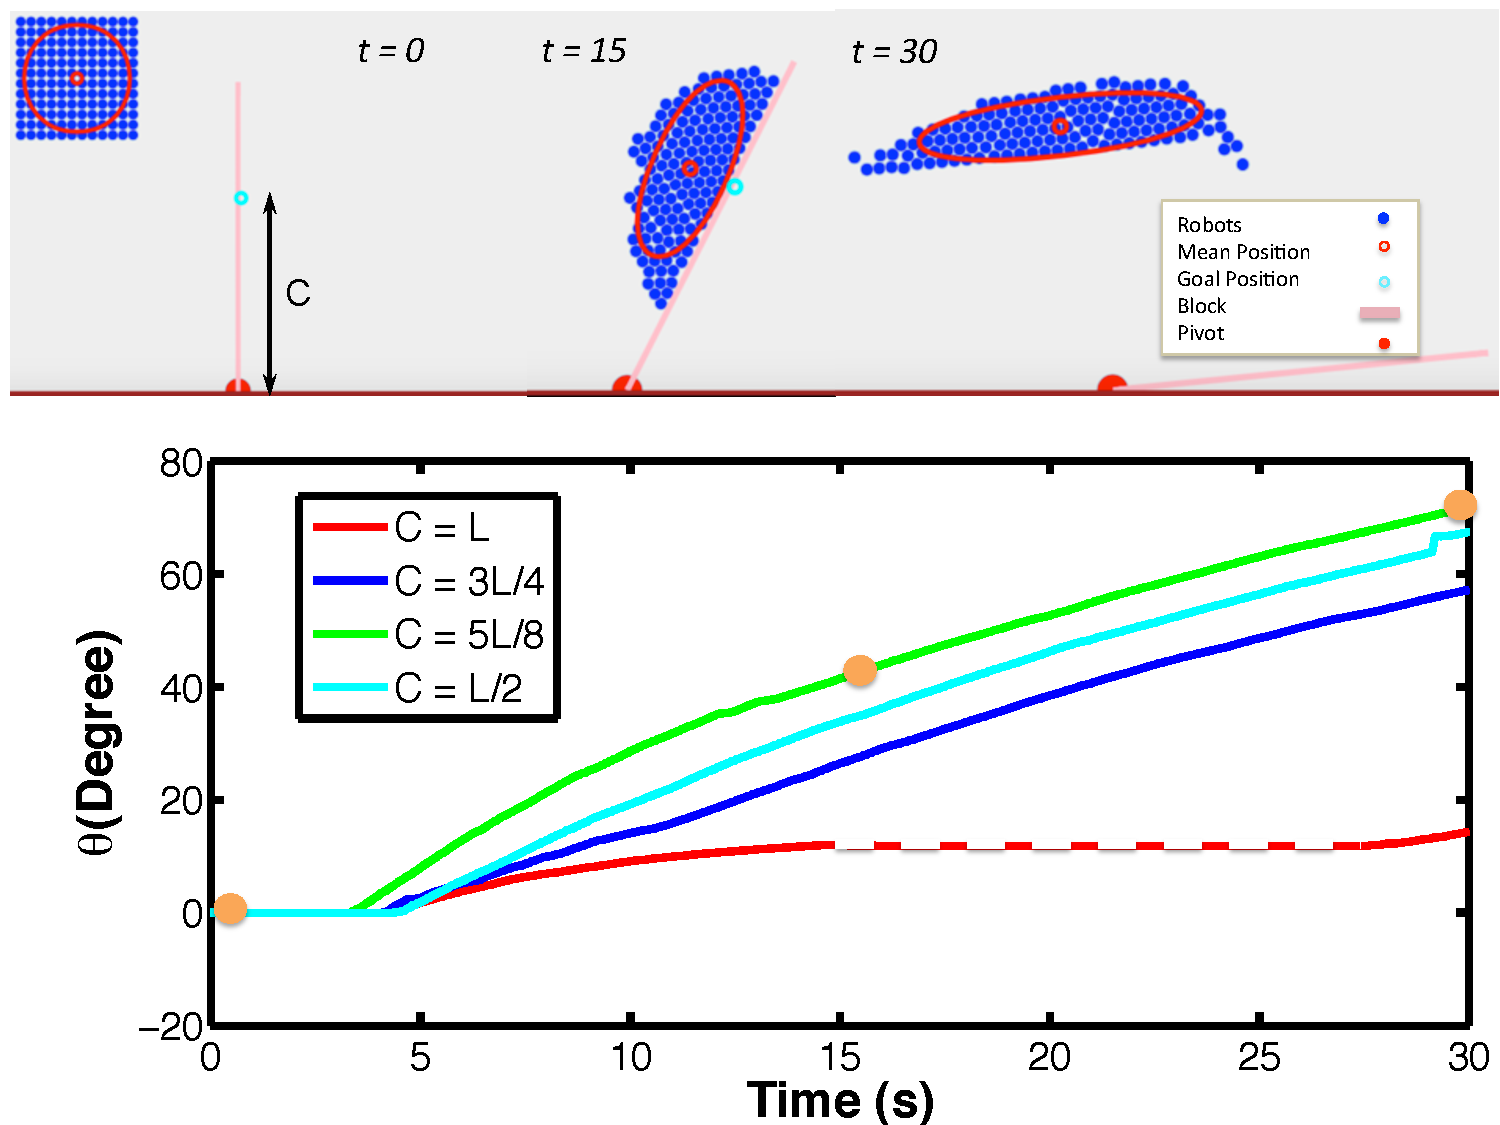
\includegraphics[width=0.8\columnwidth]{LFig.pdf}
\end{center}
\vspace{-1em}
\caption{\label{fig:LFig}
Simulation results from a swarm applying force to a hinged door. 
The swarm mean is steered toward a point $C$ units along the object from the pivot point. The red dashed line indicates the times that the swarm was in variance control mode.
 Simulation used 144 robots of diameter $0.2$ m with a standard deviation of less than $1.5$ m and an object length of $6$ m.
}
\vspace{-1em}
\end{figure}


\paragraph{Orientation of the object}
These simulations used a uniform density rectangle as the object. This object was 30$\times$ larger than the robots.
Using the pure torque control discussed in the previous paragraph, the orientation of the object can be controlled by applying force. 
The rectangular object is not pivoted, so it moves in addition to rotating. 
 The swarm still may split into multiple components.
  We use the hysteresis variance control from \cite{ShahrokhiIROS2015}  to gather the swarm when its variance grows too large. 
  The following control law chooses a goal position to regulate the orientation of the object.  
  
 \begin{align}\nonumber
goal_x = O_x +  K_{orient}  (O_{\theta} - goal_\theta ) \cos(O_{\theta}) \\
goal_y = O_y +  K_{orient}  ( O_{\theta} -goal_\theta  ) \sin(O_{\theta})
\end{align}
Here $K_{orient}$ is a positive gain on the control input.  


\begin{figure}
\begin{center}
	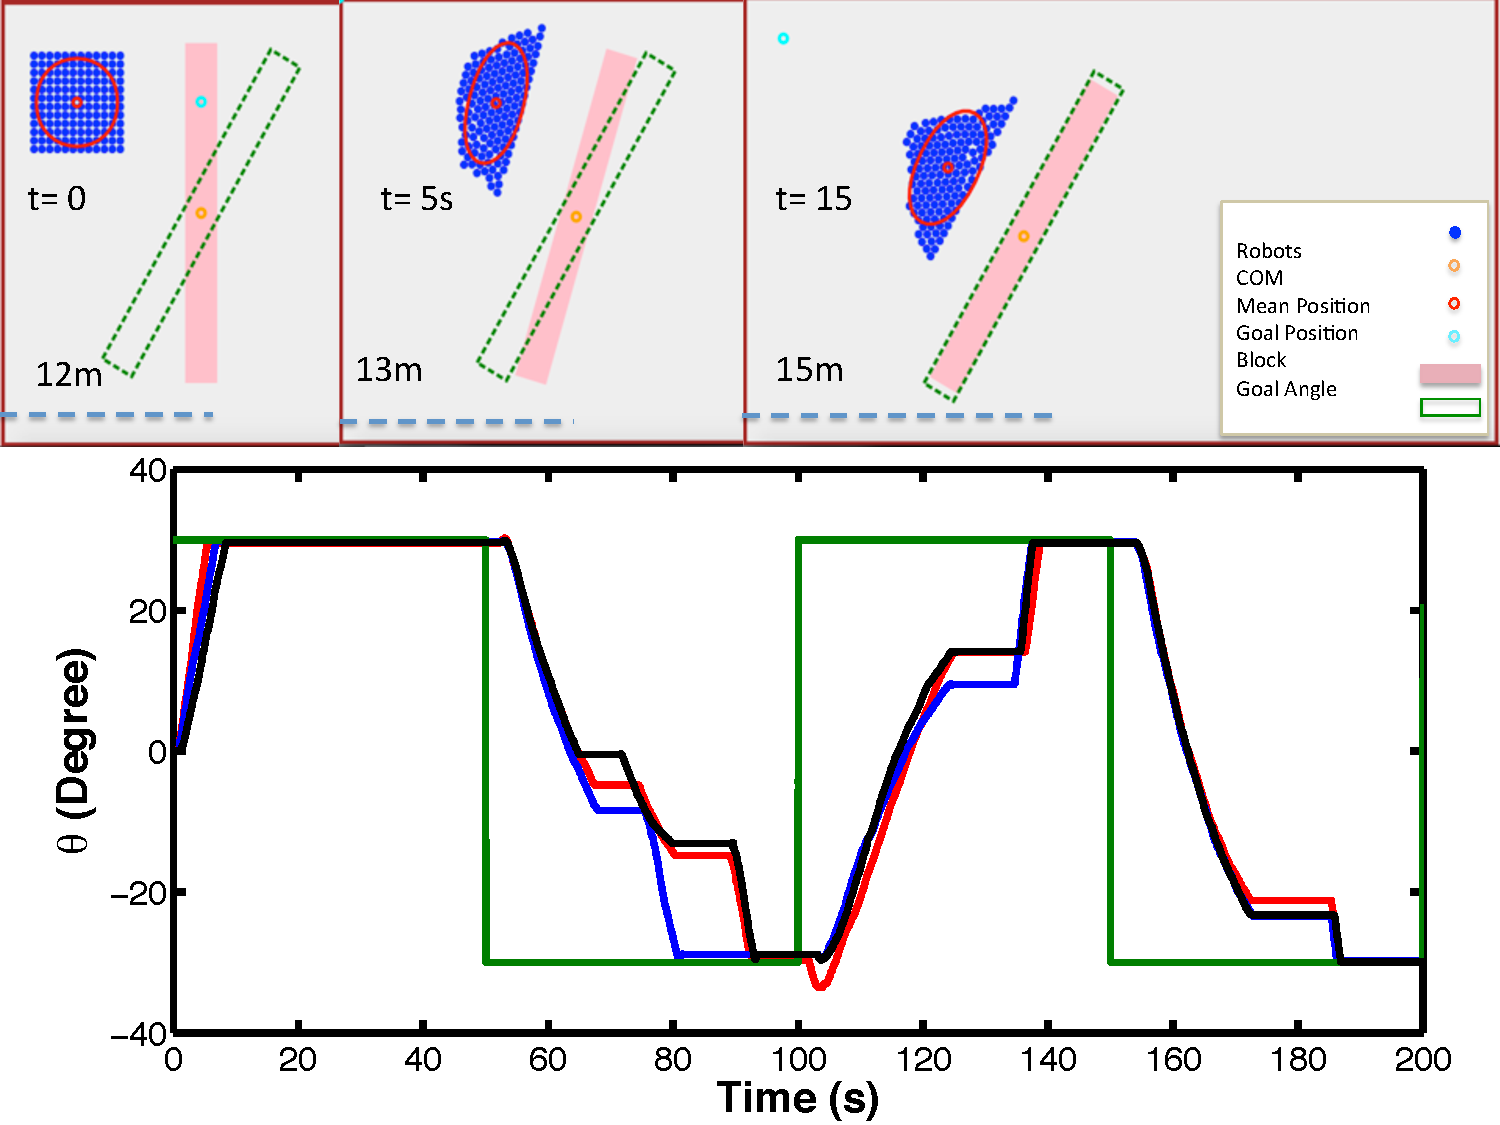
\includegraphics[width=0.8\columnwidth]{Orientation.pdf}
\end{center}
\vspace{-1em}
\caption{\label{fig:OrientCont}
Plot demonstrating  orientation control of a rectangular object. The green line is the goal orientation. Other lines show different random starting position of the swarm. When the plot traces are constant the swarm is no longer pushing the object and instead is being regathered in a corner of the workspace until the variance is below a desired threshold. 
}
\vspace{-1em}
\end{figure}

Fig. \ref{fig:OrientCont} illustrates this controller with different starting positions. When the plot traces are constant the swarm is no longer pushing the object and instead is being regathered in a corner of the workspace. Code is available at \cite{Shahrokhi16Orient}.

\paragraph{Straight translation while regulating object orientation} \label{para:PureTranslation}

When the total force is applied perpendicular to the object and in line with the center of mass, according to Eq. \eqref{eq:torque} there will be no torque. 
The following goal position for the mean position of the swarm regulates the object's orientation using $\Delta_{\theta}$ for proportional feedback  to determine where to apply force.
$\Delta_\theta = goal_\theta - O_\theta$ is the difference between the goal angle and the current object angle.
 $K_\tau$ is a constant and is tuned manually to $10$. $(O_x,O_y)$ is the position of the object's COM.
\begin{align}
goal_x &= O_x \nonumber \\
goal_y &= K_\tau \Delta_{\theta} + O_y  \label{eq:TranslationAndOrientation}
\end{align}

 Fig. \ref{fig:Straight} shows how $\Delta_{\theta}$ converges to zero with different initial configurations of the swarm. When the swarm is above or below the object it applies a torque to the object. Code is available at \cite{Shahrokhi16translation}.
 
 
\begin{figure}
\begin{center}
	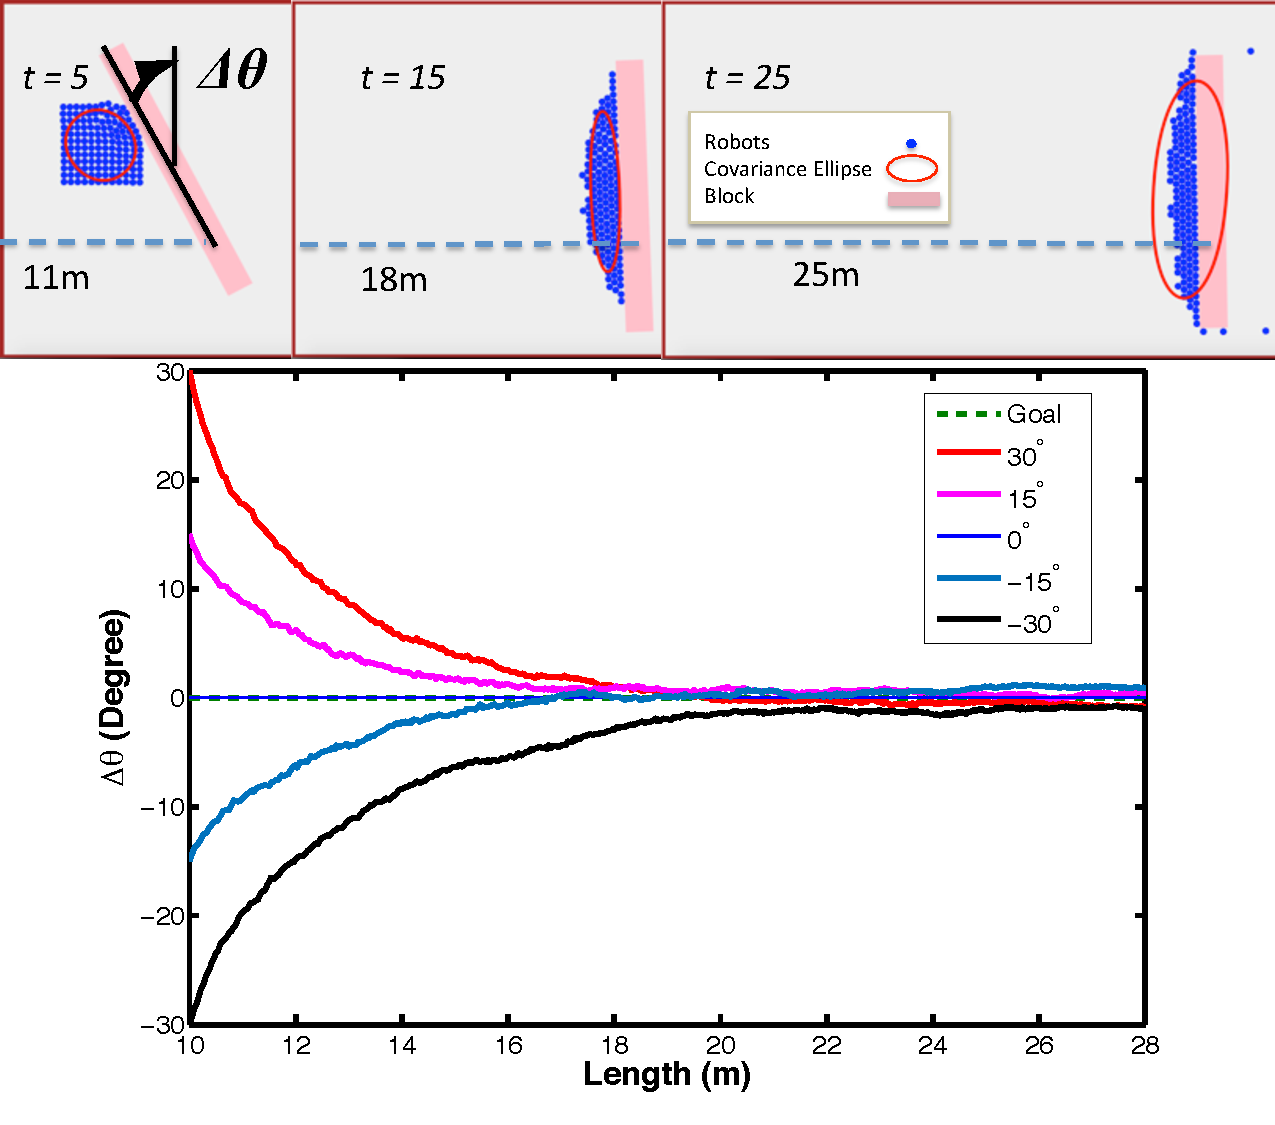
\includegraphics[width=0.8\columnwidth]{Straight.pdf}
\end{center}
\vspace{-1em}
\caption{\label{fig:Straight}
In this task, the swarm pushed the object in the $+x$ direction while trying to regulate the orientation to $goal_{\theta} = 0^\circ$.
 The swarm can push the object without changing its orientation only if it pushes along a line intersecting the COM of the object.  A feedback control law regulates the object's orientation.
}
\vspace{-1em}
\end{figure}

\paragraph{Line following with perpendicular orientation} \label{para:PureTranslation}
This task designs a control law that, given an arbitrary line, will push an object's COM onto that line and regulate the object's orientation to be perpendicular to that line.
Any line can be parameterized in the form $ax+by+c =0$,  which gives the locus of $(x,y)$ points along the line.  The point on this line nearest to the swarm COM $(O_x,O_y)$ is $P$:

%Assume an arbitrary line that if the object face that direction, the swarm should apply perpendicular force to the object to get to the desired location with the desired orientation.  We want to keep the object on the trajectory while the orientation of the object is also kept as desired. For this purpose, we have to find the intersection of the object orientation axis and the line. If the equation of the line is $ax+by+c =0$, and we name this point $P$, it can be found as:

\begin{align}
P_x &= \frac{b(bO_x-aO_y)-ac}{a^2 + b^2},\\ \nonumber
P_y &= \frac{a(-bO_x+aO_y)-bc}{a^2 + b^2}
\end{align}

%Then for keeping the object on trajectory, we will have the following goal position for correcting both perpendicular error and angle error while pushing the object:

The following control law regulates the goal position for the swarm's mean to push the object COM onto the line and regulates the object's angle.

\begin{align}
goal_x &= O_x+ K_p (O_x-P_x)+ K_\tau \frac{O_x-P_x}{||O_x-P_x||}\Delta_{\theta} \nonumber \\
goal_y &= O_y+ K_p (O_y-P_y)+ K_\tau \frac{O_y-P_y}{||O_y-P_y||}\Delta_{\theta} \label{eq:Regulate}
\end{align}

Fig. \ref{fig:Linear} shows the position and orientation over time 
while line following with perpendicular orientation.
The goal position for the swarm is based on the nearest point from COM to the line.
 %Fig. \ref{fig:LinearScreenShots} contains screenshots of this simulation. 
 Code is available at \cite{Shahrokhi16TorqueLine}.

\begin{figure}
\begin{center}
	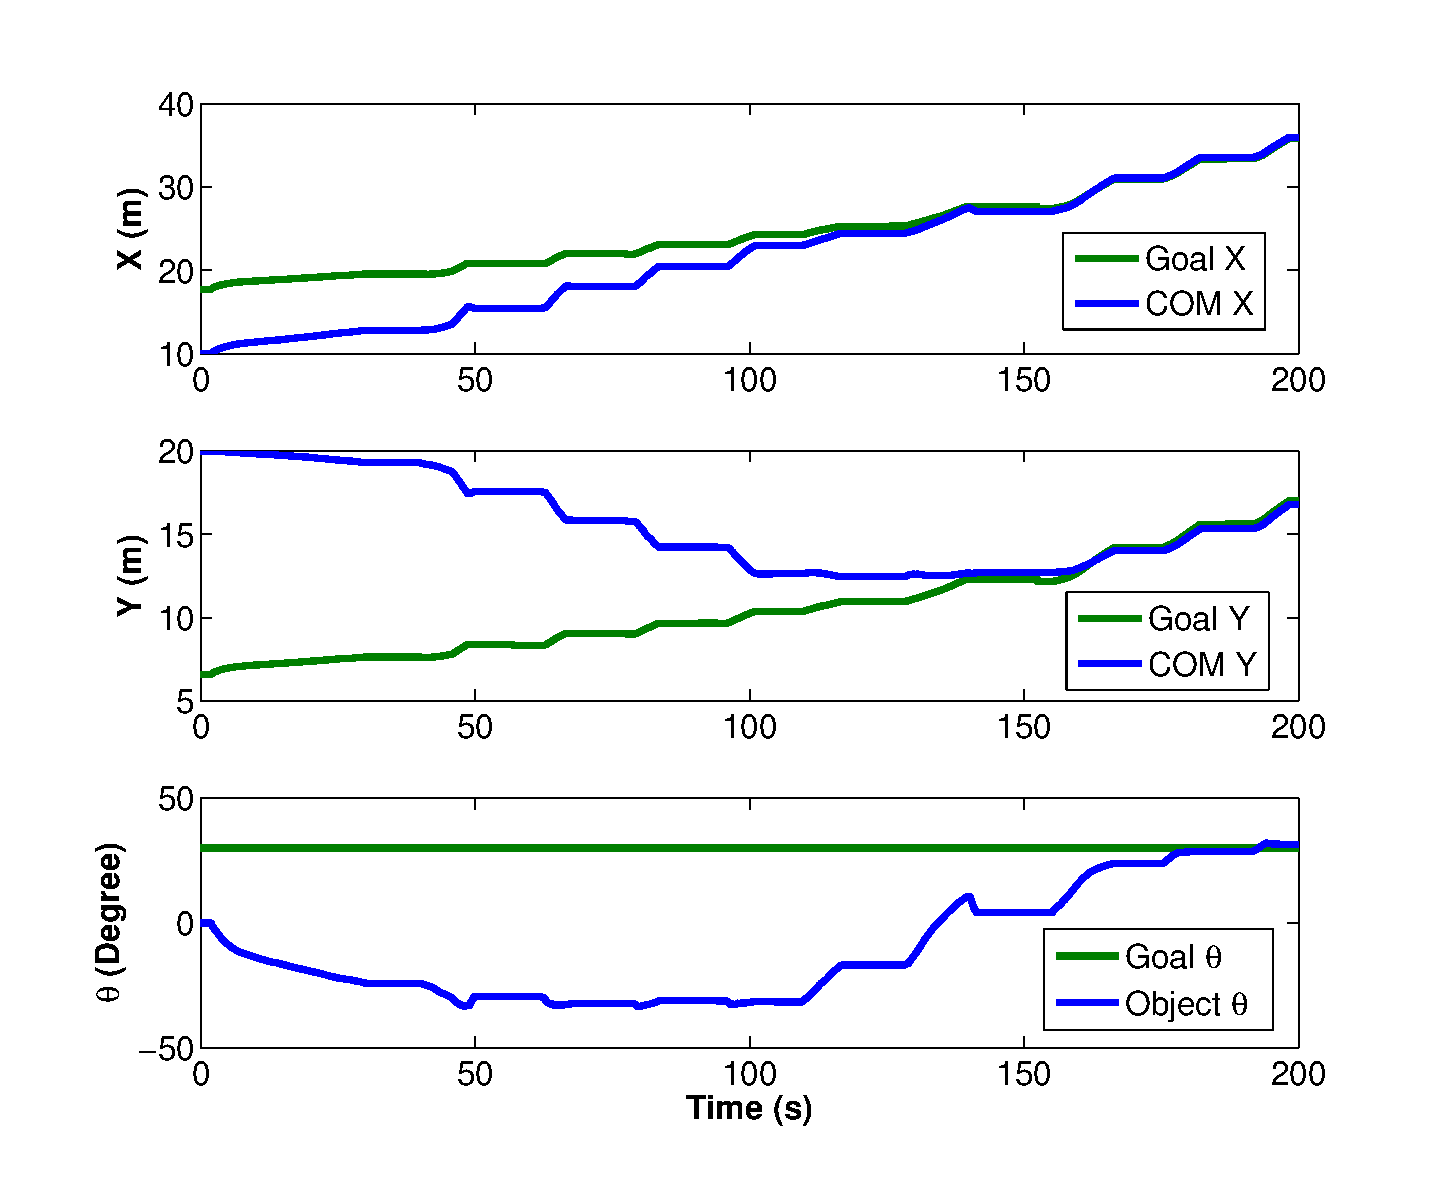
\includegraphics[width=0.75\columnwidth]{Linear.eps}
\end{center}
\vspace{-2em}
\caption{\label{fig:Linear} 
Following an arbitrary line with perpendicular orientation. This control law centers the object to the line, while it regulates its orientation.
}
\vspace{-1em}
\end{figure}


%\begin{figure*}
%\centering
%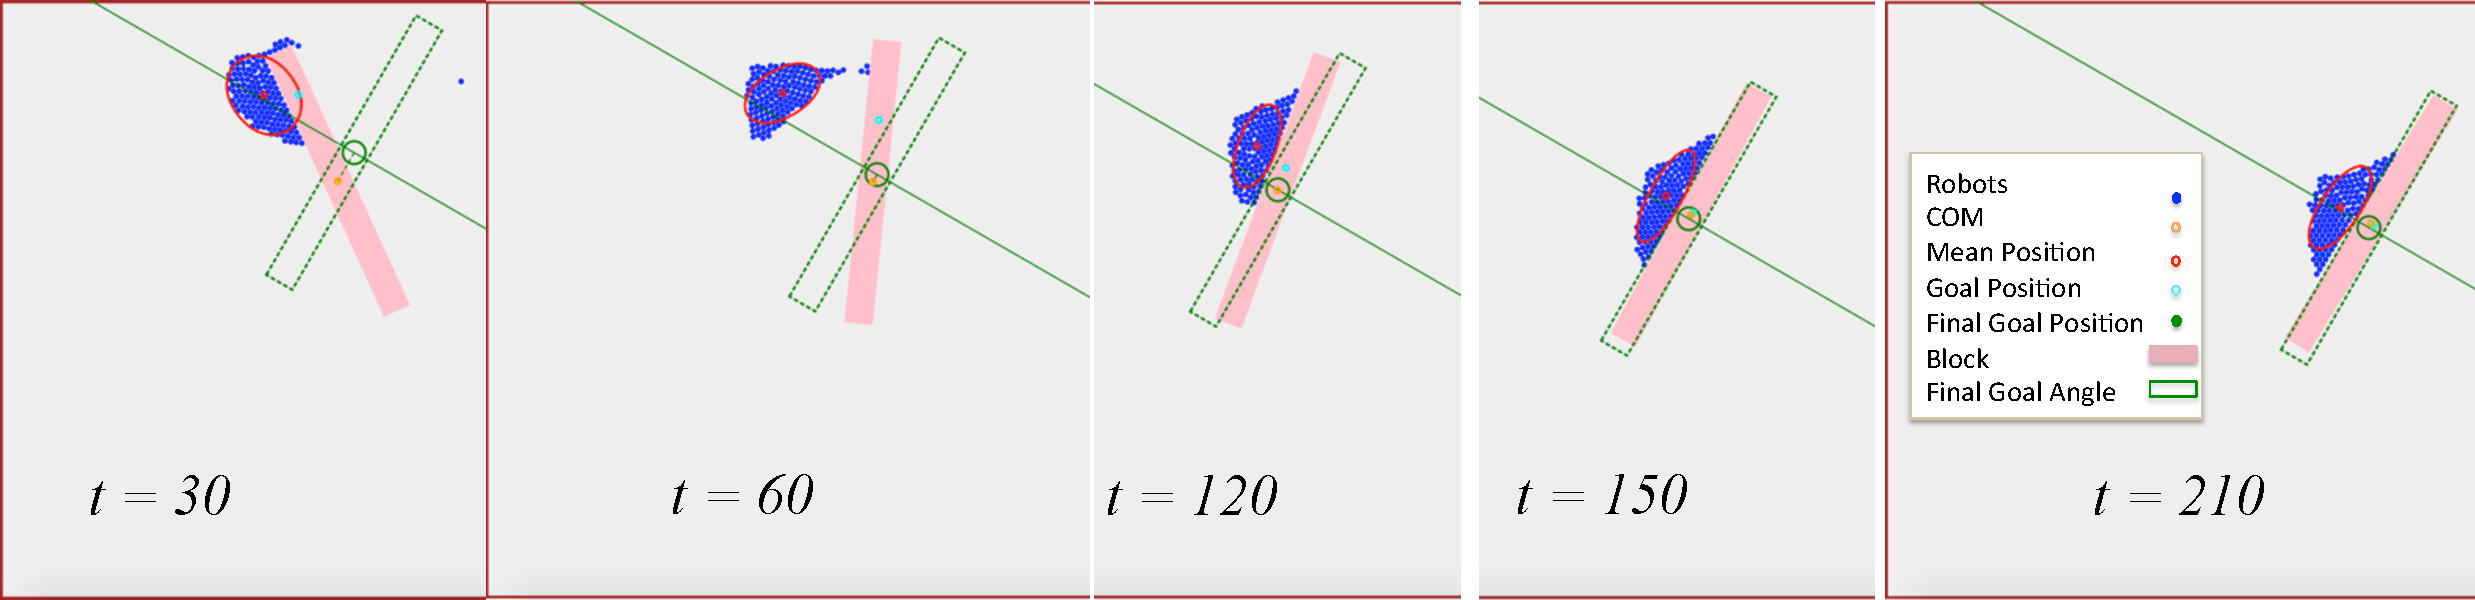
\includegraphics[width=2\columnwidth]{Linear.pdf}
%\vspace{0em}
%\caption{\label{fig:LinearScreenShots}
%Screenshots from simulation of line following with perpendicular orientation.
 %The object's COM is pushed to the line, while its orientation is regulated to be perpendicular to the line.
%}
%\end{figure*}
%TODO:  control law regulating distance from the straight line trajectory AND object orientation

%Perhaps: assume without loss of generality that the desired trajectory is the line $y = goal_y$

%\begin{align} \label{eq:StraightTrajectoryAndOrientation}
%goal_x &= O_x \nonumber \\
%goal_y &= O_y + K_\tau \Delta\theta  + K_p (O_y -  goal_y)
%\end{align}


%Shiva, you can do better than this, and write an equation to make the swarm follow an arbitrary line




\paragraph{Object pose control}
This section presents two algorithms designed to control the \emph{pose}, the position and orientation, of an object.  
Each works by first controlling the orientation and then regulating that orientation while translating the object. 

\begin{figure}
\begin{center}
	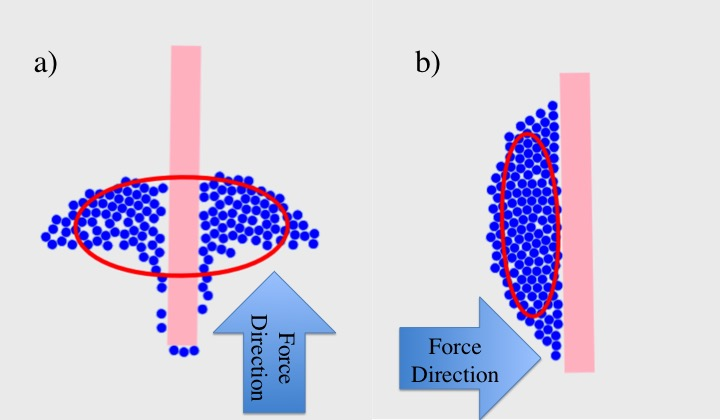
\includegraphics[width=.7\columnwidth]{perpendicular.jpg}
\end{center}
\vspace{-1em}
\caption{\label{fig:perpendicular} 
a.) Pushing an object perpendicular to its minor axis. The swarm spreads around the object. b.)  Applying force perpendicular to the object's long axis reduces the probability of splitting the swarm.
}
\vspace{-1em}
\end{figure}

The na\"{i}ve approach is represented in Alg. \ref{alg:naivePoseControlApproach}. It defines  the coordinate frame such that $[goal_x, goal_y, goal_{\theta}] = [0,0,0]$.
Then it cycles between regulating the angular error below some threshold $T_{\theta}$,
pushing the object along the major axis until position error perpendicular to the major axis is less than $T_x$, then pushing perpendicular to the minor axis until error perpendicular to the minor axis is less than $T_y$. 
This na\"{i}ve approach works poorly on objects with large aspect ratios because the swarm flows past the object, as shown in Fig.~\ref{fig:perpendicular}. 
Instead Alg. \ref{alg:PoseControl} seeks to always push the object perpendicular to the major axis, preventing the swarm from flowing around. 


\begin{algorithm}
\caption{PerpendicularPushesPoseControl}\label{alg:naivePoseControlApproach}
\begin{algorithmic}[1]
\Require $goal_x, goal_y, goal_{\theta},O_x, O_y, O_{\theta}$.
\State Define coordinate frame such that $[goal_x, goal_y, goal_{\theta}]^\top = [0,0,0]^\top$
\While {$\lvert O_x \rvert >T_x \vee \lvert O_y \rvert >T_y \vee \lvert O_{\theta} \rvert >T_{\theta}$}
	\While {$\lvert O_{\theta} \rvert >T_{\theta}$}
		\State Orientation control \S\ref{sec:simulation}.a
	\EndWhile
	\While {$\lvert O_x \rvert >T_{x}$}
		\State Straight translation \S\ref{sec:simulation}.c along line $y = 0$
	\EndWhile
	\While {$\lvert O_y \rvert >T_{y}$}
		\State Straight translation \S\ref{sec:simulation}.c along line $x = 0$
	\EndWhile
\EndWhile
\end{algorithmic}
\end{algorithm}



\begin{algorithm}
\caption{PoseControl}\label{alg:PoseControl}
\begin{algorithmic}[1]
\Require $goal_x, goal_y, goal_{\theta},O_x, O_y, O_{\theta}, C<1$.
\State $a = \cos(goal_{\theta})$ \Comment{Line Equation}
\State $b = \sin(goal_{\theta})$
\State $c = -a \cdot goal_x - b \cdot goal_y$

\Repeat 
\State $P_x = \frac{b(bO_x-aO_y)-a\cdot c}{a^2 + b^2}$  \Comment{Nearest point on line}
\State $P_y = \frac{a(-bO_x+aO_y)-b\cdot c}{a^2 + b^2}$
\State $\theta_t = goal_{\theta}+\pi/2$
\State $a_t = \cos(\theta_t )$ \Comment{Line Equation}
\State $b_t = \sin(\theta_t )$
\State $c_t = -a_t \cdot P_x - b_t \cdot P_y$
\State Line following with perpendicular orientation on line $(a_t,b_t,c_t)$  \S\ref{sec:simulation}.d
\State $d = \sqrt{(P_x-O_x)^2 + (P_y-O_y)^2}$
\Until {$d < C $} \Comment{Reaching near the line}
\State Line following with perpendicular orientation on line $(a,b,c)$ \S\ref{sec:simulation}.d
\end{algorithmic}
\end{algorithm}


Given a goal pose for the object, the algorithm constructs the line perpendicular to the long axis that intersects the goal pose. Alg.~\ref{alg:PoseControl} first moves the object to this line using the control law from \S\ref{sec:simulation}.d, then pushes the object to the goal pose using \S\ref{sec:simulation}.d.
%The swarm pushes the object to an intermediate location, from where a ``Line following with perpendicular orientation" move can deliver the object to the goal pose. 
A hysteresis-based variance control is used.  Whenever the swarm variance is bigger than a maximum variance threshold, the swarm is steered to  a corner to regather itself. 
This causes delays, but it usually prevents robots from flowing around the object. However, there is still some probability that a part of the swarm appears in front of the object, as shown in Fig. \ref{fig:PosControlFig} where at $t\approx170$ the orientation of the object is affected when the swarm is trying to regather because several robots were in front of the object. Fig. \ref{fig:PosScreenShot} shows screenshots of the simulation. Simulation code that runs natively in any modern web browser is available at \cite{Shahrokhi16pose}.

\begin{figure}
\begin{center}
	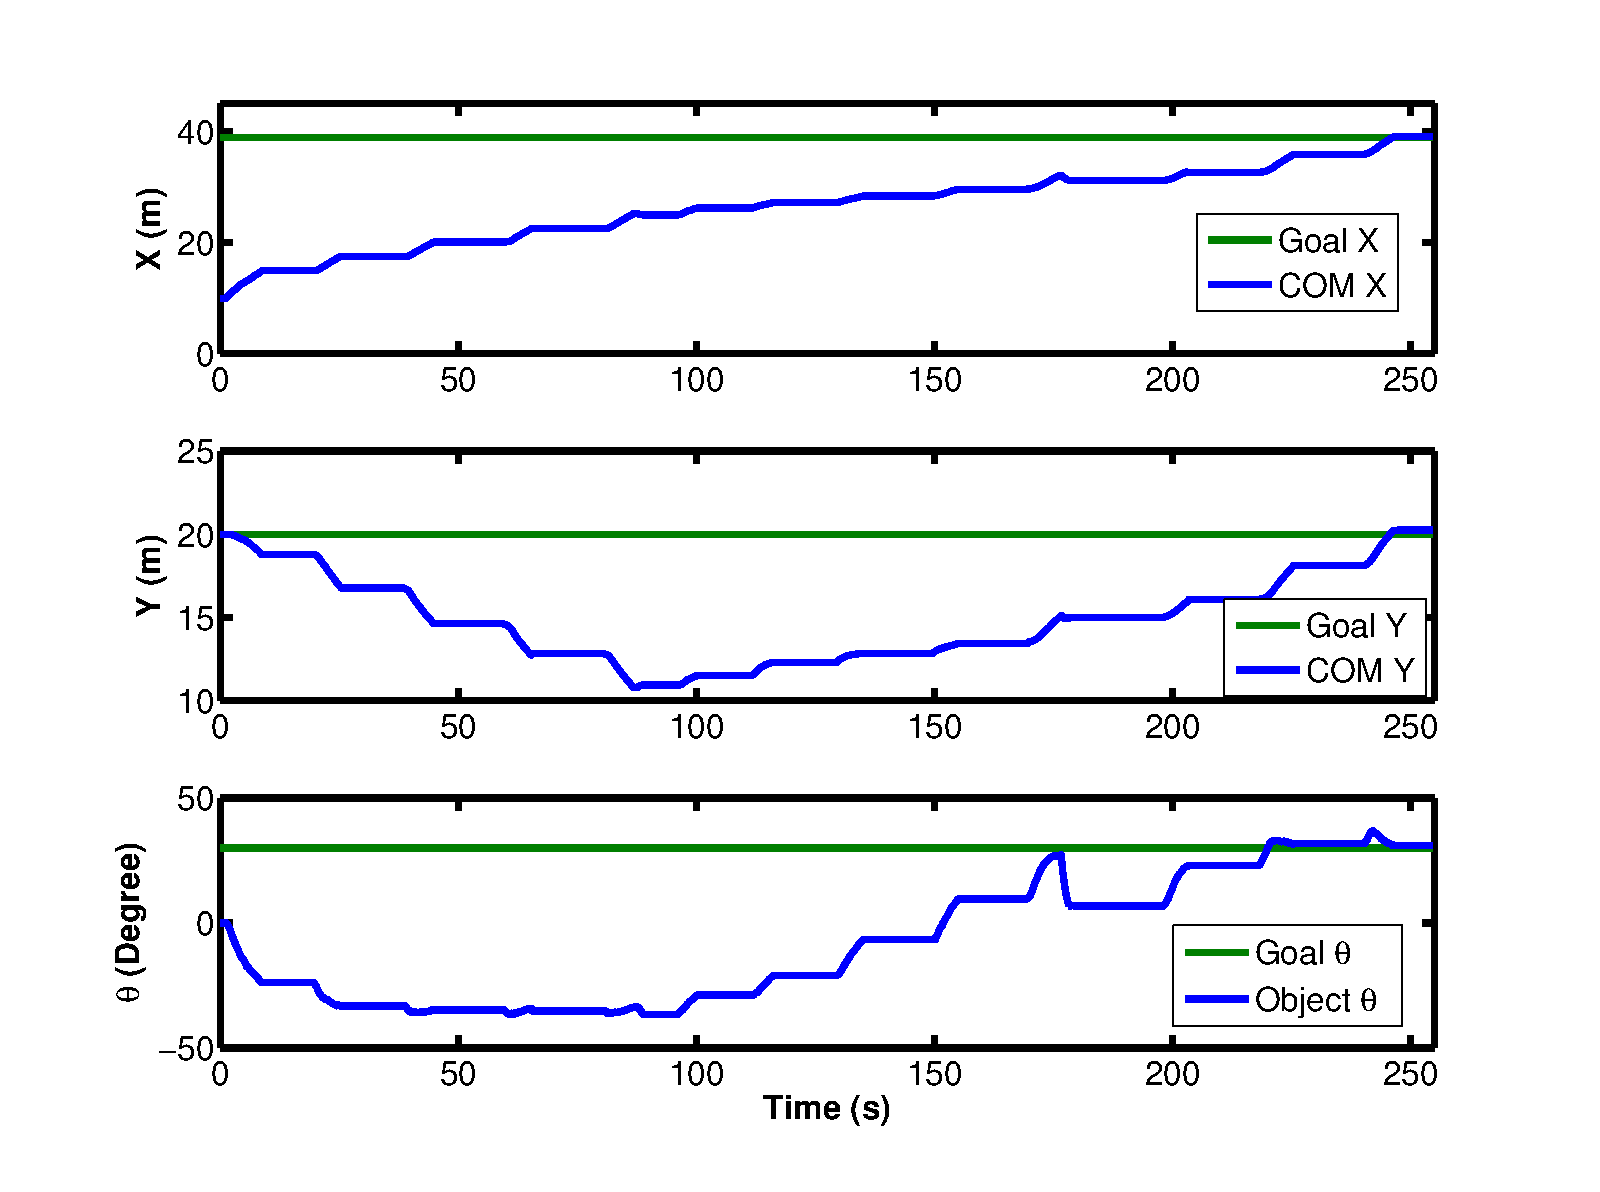
\includegraphics[width=0.9\columnwidth]{PosControl.eps}
\end{center}
\vspace{-2em}
\caption{\label{fig:PosControlFig} 
Pose control using Alg. \ref{alg:PoseControl}.  The objects is delivered to a goal position and orientation. The parts that the position including orientation is not changing, the swarm is in variance control mode to avoid splitting as much as it is possible. 
}
\vspace{-1em}
\end{figure}


\begin{figure*}
\centering

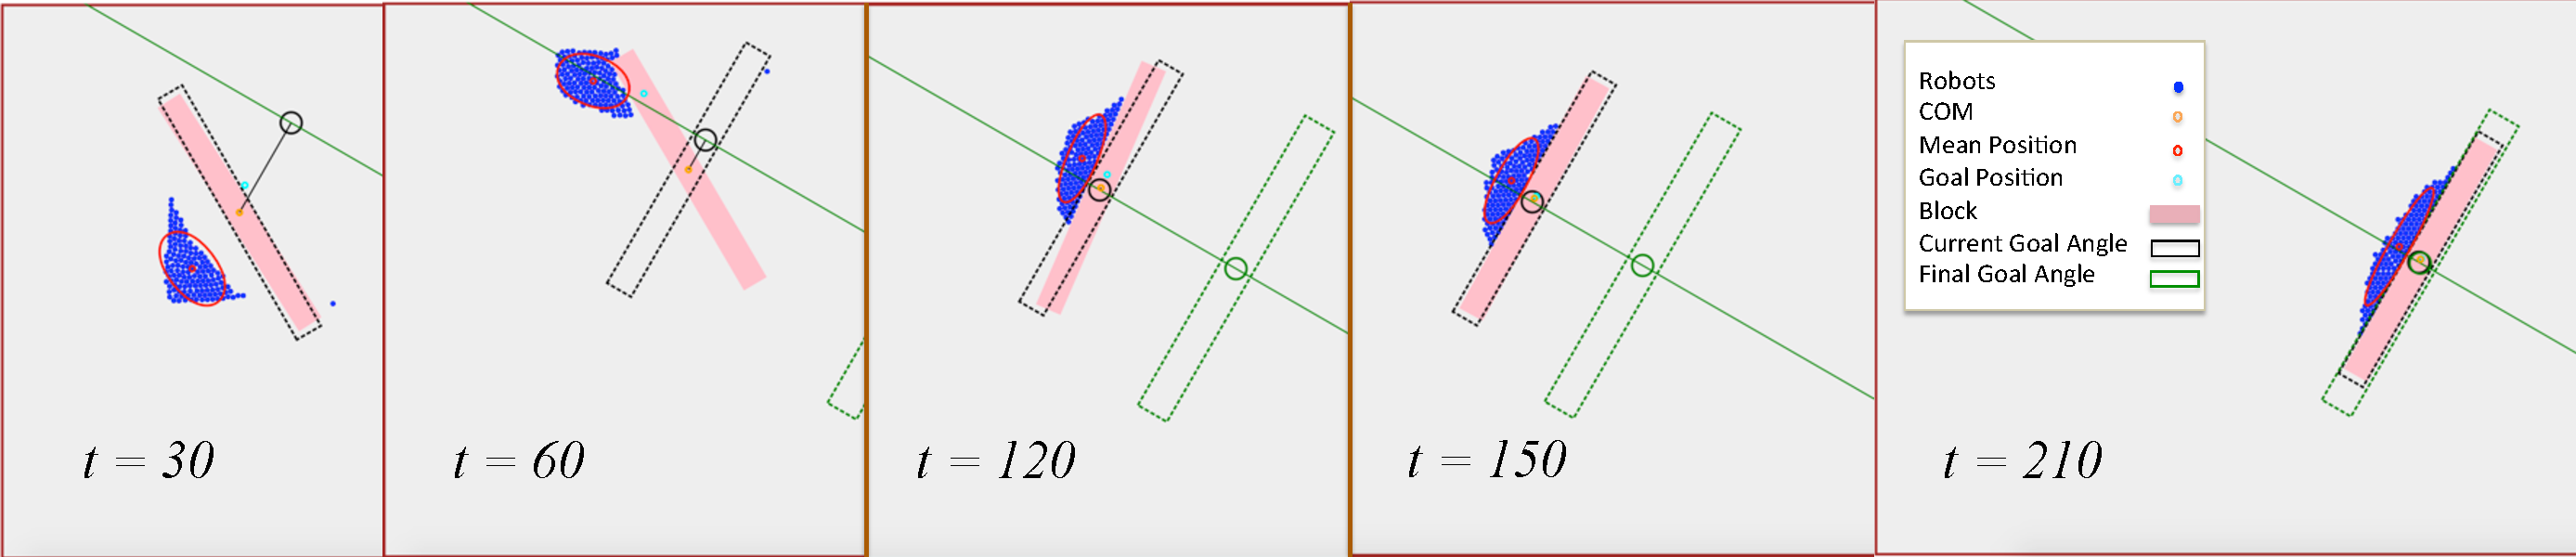
\includegraphics[width=1.6\columnwidth]{PoseControl.pdf}
\vspace{0em}
\caption{\label{fig:PosScreenShot}
Different stages for position control of a block while controlling its orientation. The first task (0--90 s) is to push the object COM to a line perpendicular to the goal. The second task (90--210 s) is to push the object along this perpendicular line while regulating the orientation.
}
\end{figure*}



%%%%%%%%%%%%%%%
%%%%%%%%%%%%%%%

%%%%%%%%%%%%%%%%%%%%%%%%%%%%%%%%%%%%%%%%%%%%%%%%%%%%%%%%%%%
\section{Experiment}\label{sec:expResults}
%%%%%%%%%%%%%%%%%%%%%%%%%%%%%%%%%%%%%%%%%%%%%%%%%%%%%%%%%%%



%\subsection{Hardware System}


Our experiments are on centimeter-scale hardware systems called \emph{kilobots}.  These allows us to emulate a variety of dynamics, while enabling a high degree of control over robot function, the environment, and data collection. The kilobot, from \cite{Rubenstein2012,rubenstein2014programmable} is a low-cost robot designed for testing collective algorithms with large numbers of robots. It is available as an open source platform or commercially from~\cite{K-Team2015}.  Each robot is approximately 3 cm in diameter, 3 cm tall, and uses two vibration motors to move on a flat surface at speeds up to 1 cm/s.  Each robot has one ambient light sensor that is used to implement \emph{phototaxis},  moving towards a light source. 
In these experiments as shown in Fig.~\ref{fig:setup}, we used $n$=97 kilobots, a glass-covered 1.5 m$\times$1.2 m whiteboard as the workspace, and eight 30W LED floodlights arranged 1.5 m above the plane of the table at the $\{N,NE,E,SE,S,SW,W,NW\}$ vertices of a 6 m square centered on the workspace. The lights were controlled using an Arduino Uno board connected to an 8-relay shield.  Above  the table, an overhead machine vision system tracks the position of the swarm.


\begin{figure}
\begin{center}
	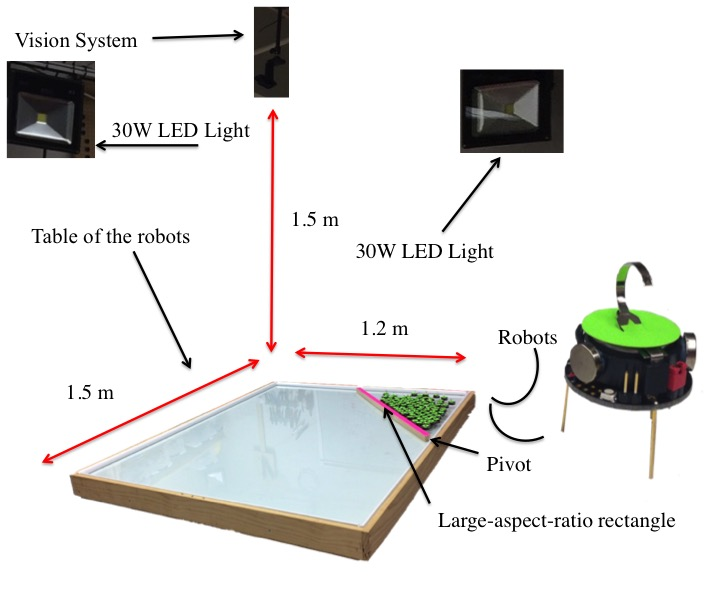
\includegraphics[width=.9\columnwidth]{SetUp.jpg}
\end{center}
\vspace{-1em}
\caption{\label{fig:setup}
Hardware platform:  table with 1.5$\times$1.2 m workspace, surrounded by eight remotely triggered 30W LED floodlights, with an overhead machine vision system.
}
\vspace{-1.5em}
\end{figure}

The experiments from Section \ref{sec:simulation}.a were repeated using this physical swarm.
Fig. \ref{fig:expBig} illustrates an experiment showing pure torque control with a swarm of robots. In this figure a large-aspect-ratio rectangle  (91$\times$2 cm, colored pink in the image) was hinged to one side of the table.  Like a door, this object could only be moved around this pivot. 
Two trials were performed.  In each trial the swarm was initialized in the lower right side of the table, and then commanded to push the object with the mean position of the swarm directed toward a point distance $C$ from the pivot point. Data was recorded for 150 seconds.
In the first trial, $C = L$, so the robots were commanded to push the door at the extreme edge of the door from the pivot.  
In the second trial $C = 1/2 L$, and so the swarm pushed the object in the center of the rectangle.
As discussed in Section \ref{sec:simulation}, the robots spread when commanded to push the object at the extreme end, and half of the robots flowed past the end of the rectangle without engaging the rectangle.
 This illustrates a key difference between robotic swarms and a single pusher robot. The swarm exerts the most torque when  \eqref{eq:swarmtorque} is maximized.
  \eqref{eq:swarmtorque} is maximized when the majority of the swarm engages the object.
For this reason in Fig. \ref{fig:expBig}, the trial in the second row of screenshots moves the door further than the  trial in the  first row.
\begin{figure*}
\centering

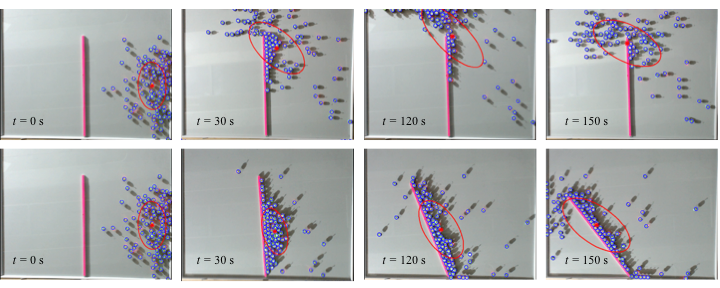
\includegraphics[width=2\columnwidth]{Experiment.png}
\vspace{-1em}
\caption{\label{fig:expBig}{Snapshots showing the effect of pushing a pivoted rectangular object at different distances from the pivot point. 
 97 robots were programmed to move toward the brightest light in the room, and   controlled by choosing which of 8 lights were on at any given instant. The top row of snapshots illustrate the swarm pushing at the end of the object.  In this case,  the swarm flows past the object and the force decreases. The bottom row illustrates that when the swarm pushes at the middle of the object the force provided by the swarm remains constant. In this case the swarm does not flow past the object. See video attachment for recordings of these experiments at\href{https://www.youtube.com/watch?v=ZiKEa5UwukM&feature=youtu.be}{\cite{ShahrokhiTorqueVideo}}.
 }
%\vspace{-2em}
}
\end{figure*}







%%%%%%%%%%%%%%%
%%%%%%%%%%%%%%%
%%%%%%%%%%%%%%%%%%%%%%%%%%%%%%%%%%%%%%%%%%%%%%%%%%%%%%%%%%%
\section{Conclusion and Future Work}\label{sec:conclusion}
%%%%%%%%%%%%%%%%%%%%%%%%%%%%%%%%%%%%%%%%%%%%%%%%%%%%%%%%%%%


This paper presented techniques for controlling the orientation of an object by manipulating it using a swarm of simple robots with global inputs.
The paper provided algorithms for precise orientation control, as well as demonstrations of orientation control. 


Future efforts should be directed toward optimizing torque control, applying the techniques to hardware robots, pose control for multiple part assembly, and manipulation in a crowded workspace.
The control laws in this paper used only the mean and variance of the swarm.  The control techniques may be optimized using high-order moments, or by stochastic modeling of the collisions between swarm members and the object.

%TODO JOURNAL: design controllers that efficiently regulate $\sigma_{xy}$.
%TODO JOURNAL: We will design Lyapunov-inspired controllers for $\sigma_{xy}$ to prove controllability. 
%TODO JOURNAL:  and rank controllability as a function of friction.
% TODO: JOURNAL: and vary wall friction by laser-cutting boundary walls with a variety of profiles. 


%    Inspired by large-scale human experiments with swarms of robots under global control,  this paper investigated controllers that use only the mean and variance of a robot swarm. We proved that the mean position is controllable, and provided conditions under which variance is controllable.  We derived automatic controllers for each and a hysteresis-based switching control that controls the mean and variance of a robot swarm.  We employed these controllers as primitives for a block-pushing task. 
%    
%    Future work should implement these controllers on a robot swarm and decrease completion time by avoiding counter-productive contact with the block while the swarm is lowering its variance.  We have also assumed the swarm is unimodal and has a straight-line path to the moveable block. Relaxing these assumptions requires solving the \emph{gathering problem}.  The gathering problem for a swarm with uniform inputs is largely unexplored, and must be examined probabilistically for nontrivial environments.
%    
    % We should also control the covariance $\sigma_xy$ and higher moments of the distribution
    
    
    
%Sensing is expensive, especially on the nanoscale. To see nanocars~\cite{Chiang2011}, scientists fasten molecules that fluoresce light when activated by a strong light source. Unfortunately, multiple exposures can destroy these molecules, a process called \emph{photobleaching}. Photobleaching can be minimized by lowering the excitation light intensity, but this increases the probability of missed detections~\cite{Cazes2001}. A control methodology based on statistics of the robot swarm rather than the actual position of each robot, allows relaxing demands on imagine systems, controllers robust to tracking errors, and a simpler methodology.  In this work we...
%


% Additionally, as population characteristics, they are available even if only a percentage of the robots are detected each control cycle.
%Photobleaching: http://www.piercenet.com/browse.cfm?fldID=4DD9D52E-5056-8A76-4E6E-E217FAD0D86B
%
%Photobleaching is caused by the irreversible destruction of fluorophores due to either the prolonged exposure to the excitation source or exposure to high-intensity excitation light. Photobleaching can be minimized or avoided by exposing the fluor(s) to the lowest possible level of excitation light intensity for the shortest length of time that still yields the best signal detection; this requires optimization of the detection method using high sensitivity CCD cameras, high numerical aperture objective and/or the widest bandpass emission filter(s) available. Other approaches include using fluorophores that are more photostable than traditional fluorophores and/or using antifade reagents to protect the fluor(s) against photobleaching. Steps to avoid photobleaching are not feasible for all detection methods and should be optimized for each method used. For example, antifade reagents are toxic to live cells, and therefore they can only be used with fixed cells or tissue. Furthermore, some detection methods, such as flow cytometry, normally do not require steps to avoid photobleaching because of the extremely short exposure time of the fluorophore to the excitation source.
%%%%%%%%%%%%%%%



%\missingfigure[figwidth=6cm]{Intro: image of real kilobots making torque to a rectangular object}
%\missingfigure[figwidth=6cm]{Theory: drawing of an object that illustrates what torque and force is}
%\missingfigure[figwidth=6cm]{Simulation: snapshots of the simulation doing torque control with blue disks}
%\missingfigure[figwidth=6cm]{Simulation: plot showing angular velocity of the object and the goal angles}
%\missingfigure[figwidth=6cm]{Experiment:plot showing angular velocity of the object and the goal angles }
%\missingfigure[figwidth=6cm]{Experiment: snapshots of the kilobots doing torque control of a rectangular object}



    
\section{Acknowledgements}
%RULES: http://www.nsf.gov/pubs/policydocs/pappguide/nsf16001/aag_6.jsp
This material is based upon work supported by the National Science Foundation under Grant No.\ 
\href{http://nsf.gov/awardsearch/showAward?AWD_ID=1553063}{ IIS-1553063}.
%Optional disclaimer (mandatory for non-scientific)
Any opinions, findings, and conclusions or recommendations expressed in this material are those of the authors and do not necessarily reflect the views of the National Science Foundation.
%We acknowledge many \href{http://mrsl.rice.edu/}{mrsl.rice.edu} lab members who helped beta test \href{http://www.swarmcontrol.net}{SwarmControl.net}; helpful discussion with \href{http://www.jmtour.com/}{James Tour}, \href{http://slink.rice.edu/}{Stephan Link}, and Victor Garc\`ia L\`opez on fabrication and visualization challenges at the nanoscale with nanocars; and the \href{http://cttl.rice.edu/}{Rice Center for Technology in Teaching and Learning}.
%This work was partially supported by the National Science Foundation under 
%\href{http://www.nsf.gov/awardsearch/showAward?AWD_ID=1035716}{CPS-1035716}.  
   
\bibliographystyle{IEEEtran}
\bibliography{IEEEabrv,TorqueControl,../../../RoboticSwarmControlLab/bib/aaronrefs}
\end{document}


%/Users/ab55/Desktop/svn/MRSL-Papers/Drafts-Current/2013-03-13-IROS-MassiveUniformManipulation/document
%/Users/ab55/Desktop/svn/ensemble/bib





